\documentclass{beamer}
\usetheme{Boadilla}
\usepackage[utf8x]{inputenc}
\usepackage{listings}
\usepackage{subfig}
%\title{LS Genio Platform}
%\subtitle{Piattaforma per il monitoraggio di macchine utensili con integrazione a software ERP Microsoft Dynamics NAV}
%\author{Vincenzo Nucci e Matteo Tiberi}
%\author{Matteo Tiberi}
%\institute{Università di Camerino}
\date{}
\begin{document}
	
	\begin{frame}
	\centering
	
\includegraphics[scale=0.25]{images/frontespizio-beamer.png}\par
	\usebeamertemplate{title page}
\end{frame}

\begin{frame}
	\frametitle{Contenuti}
	\begin{itemize}
		\item IoT \& Application development
		\item LS Genio Mash-up
		\item Streaming data visualization
	\end{itemize}
\end{frame}

\begin{frame}
	\frametitle{IoT \& Application development}
	\begin{itemize}
		\item Industria 4.0 in Logical System (Jesi) nel dominio delle aziende manifatturiere
		\item Monitoraggio delle macchine utensili in linea di produzione
		\item Necessità di piattaforme di integrazione tra applicazioni e macchine utensili (PLC)
		\item Studio e sviluppo di un mash-up per un interfacciamento trasparente tra applicazioni e PLC
	\end{itemize}
\end{frame}

\begin{frame}
\frametitle{IoT \& Application development}
	\begin{itemize}
		\item La vera potenzialità dell'IoT è la realizzazione delle sue applicazioni
		\item Data collection dai devices (PLC)
		\begin{itemize}
			\item Per l'analisi e l'apprendimento dell'environmental context (linea di produzione)
			\item Schedulazione e pianificazione dei task
			\item Aumento di qualità sia del prodotto finale che del processo produttivo
		\end{itemize}
	\end{itemize}
\end{frame}

\begin{frame}
	\frametitle{LS Genio Mash-up}
	\begin{itemize}
		\item Il mash-up indica un mix di codice, sistemi, tecnologie diverse che vengono integrate dinamicamente per creare un nuovo tipo di servizio o applicazione
		\item LS Mash-up: integrazione di diversi componenti per la creazione di una piattaforma di integrazione tra applicazioni e PLC.
	\end{itemize}
\end{frame}

\begin{frame}
\frametitle{LS Genio Mash-up}
\framesubtitle{Idea Architetturale}
%\textbf{Idea Architetturale} 
\begin{columns}[T] % align columns
	\begin{column}{.52\textwidth}
		\begin{itemize}
			\item Architettura orientata ai servizi REST
			\item Interfacce di comunicazione ben definite (JSON-ISO 19156:2011) 
			\item Subscribe per l'event listening (MOM ActiveMQ)
			\item Gestione della semantica delle misurazioni
			\item Architettura n-tier 
		\end{itemize}
	\end{column}%
	\hfill%
	\begin{column}{.48\textwidth}
		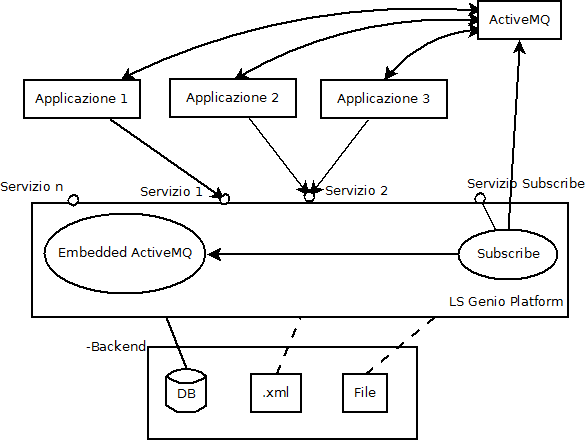
\includegraphics[width=0.9\textwidth]{images/architettura_piattaforma.png}
	\end{column}%
\end{columns}
\end{frame}

\begin{frame}
	\frametitle{LS Genio Mash-up}
	\framesubtitle{Interoperabilità tramite servizi REST}
	\begin{columns}[T] % align columns
		\begin{column}{.4\textwidth}
			\begin{itemize}
				{\tiny
					\item API tramite servizi REST
					\item Servizi disponibili
					\begin{itemize}
						\tiny
						\item getlastmeasure
						\item getmeasurefromto
						\item getdetailedmeasurefromto
						\item getmeasurelastmonth
						\item getmeasurelastweek
						\item getdetailedmeasurelastmonth
						\item getdetailedmeasurelastweek
						\item getallplc
						\item sensordatafromfields
						\item subscribe
						\item unsubscribe
					\end{itemize}
				}
			\end{itemize}
			
		\end{column}%
		\hfill%
		\begin{column}{.56\textwidth}
			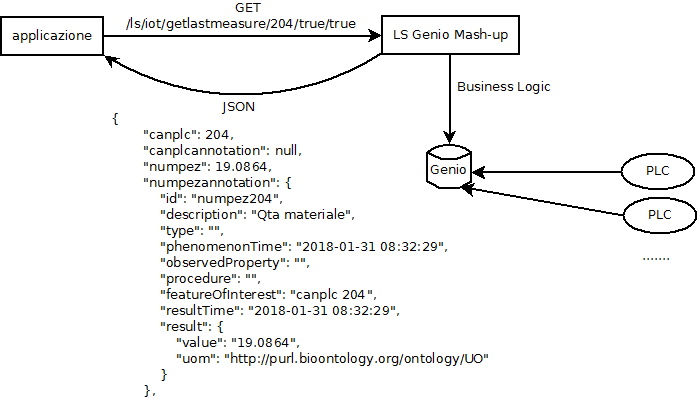
\includegraphics[width=1\textwidth]{images/interoperabilita-rest.png}
		\end{column}%
	\end{columns}
\end{frame}

\begin{frame}
\frametitle{LS Genio Mash-up}
\framesubtitle{Esempio di un servizio - getlastmeasure}
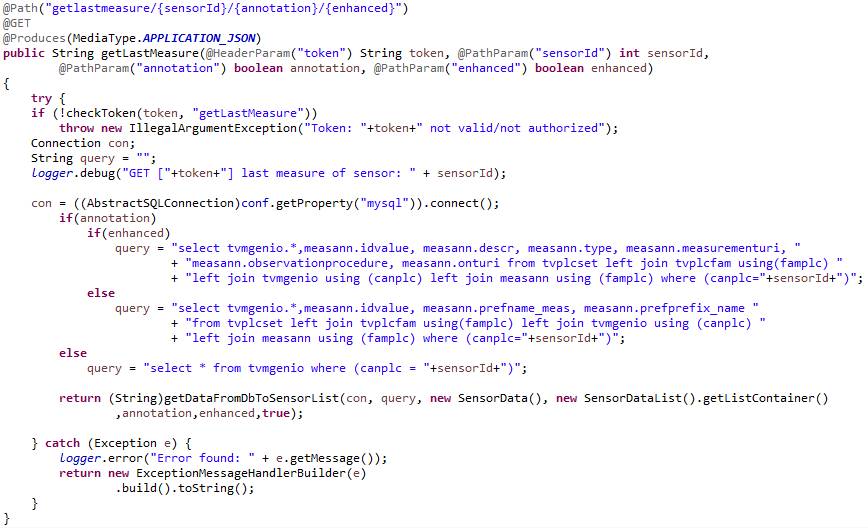
\includegraphics[width=1\textwidth]{images/getlastmeasure.png}
\end{frame}

\begin{frame}
\frametitle{LS Genio Mash-up}
\framesubtitle{Valori di ritorno di getlastmeasure}
\begin{columns}[T] % align columns
\begin{column}{.38\textwidth}
	\begin{itemize}
		\small
		\item Utilizzo di ontologie per dare semantica ai messaggi, secondo lo standard ISO 19156:2011
	\end{itemize}
	
\end{column}%
\hfill%
\begin{column}{.58\textwidth}
	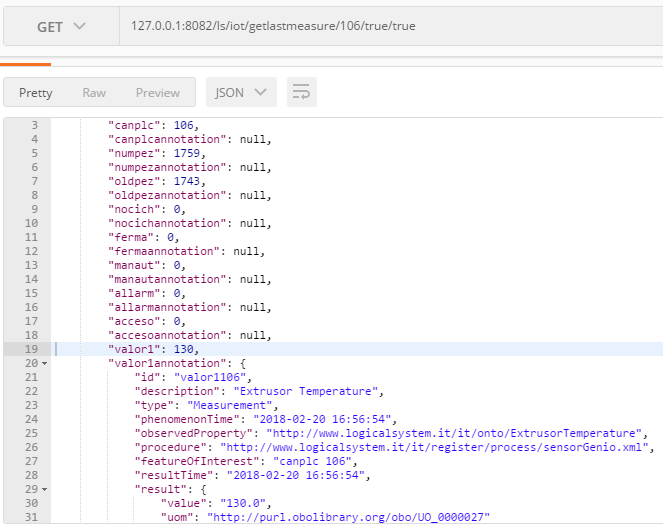
\includegraphics[width=1\textwidth]{images/Postman1-corretto.png}
\end{column}%
\end{columns}

\end{frame}

\begin{frame}
	\frametitle{LS Genio Mash-up}
	\framesubtitle{Schema servizio subscribe}
	\begin{columns}[T] % align columns
		\begin{column}{.38\textwidth}
			\begin{itemize}
				\small
				\item Invio della regola di subscribe
				\item Un thread gestisce una regola
				\item Invio dei dati in ActiveMQ quando si verifica l'evento
				
			\end{itemize}
			
		\end{column}%
		\hfill%
		\begin{column}{.60\textwidth}
			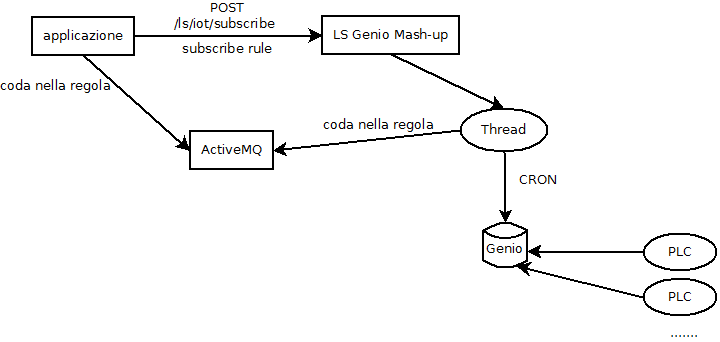
\includegraphics[width=1\textwidth]{images/schema-subscribe.png}
		\end{column}%
	\end{columns}
\end{frame}

\begin{frame}
	\frametitle{LS Genio Mash-up}
	\framesubtitle{Esempio messaggio di subscribe}
	\begin{columns}[T] % align columns
		\begin{column}{.38\textwidth}
			\begin{itemize}
				\item Regola di subscribe
				\begin{itemize}
					\item Campi del database
					\item Intervallo CRON
					\item Clausola where
				\end{itemize}
			\end{itemize}
			
		\end{column}%
		\hfill%
		\begin{column}{.58\textwidth}
			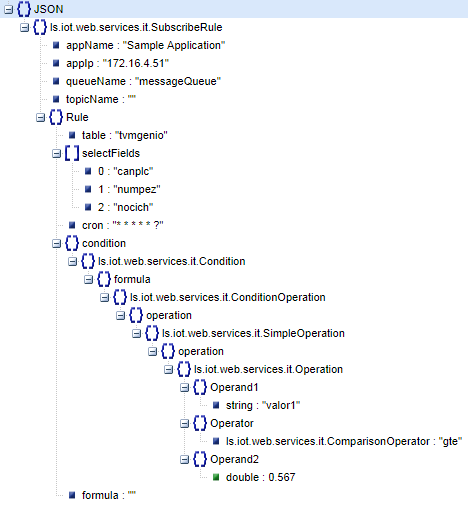
\includegraphics[width=1\textwidth]{images/subscribe-json-1.png}
		\end{column}%
	\end{columns}
\end{frame}

\begin{frame}
	\frametitle{LS Genio Mash-up}
	\framesubtitle{Albero della condition}
	\begin{columns}[T] % align columns
		\begin{column}{.26\textwidth}
			\begin{itemize}
				\tiny
				\item Suddivide la where in diversi componenti
				\begin{itemize}
					\tiny
					\item Operatori logici binari
					\item Operatori che si applicano a sotto-query
					\item Semplici operazioni
				\end{itemize}
				
			\end{itemize}
			
		\end{column}%
		\hfill%
		\begin{column}{.7\textwidth}
			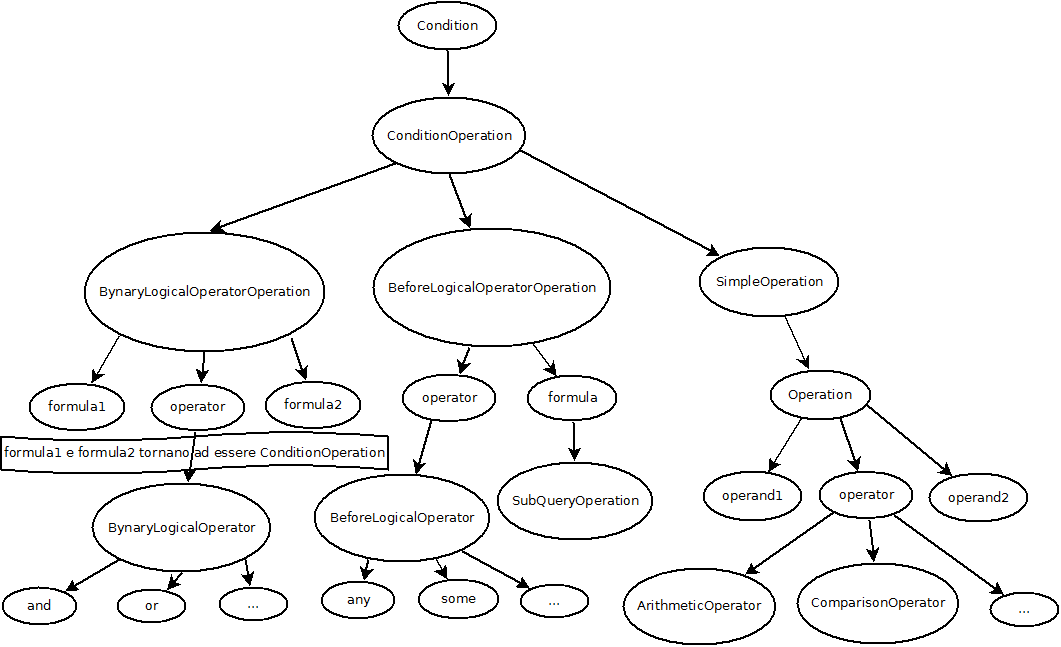
\includegraphics[width=1\textwidth]{images/strutturaquerytree.png}
		\end{column}%
	\end{columns}
\end{frame}

\begin{frame}
	\frametitle{LS Genio Mash-up}
	\framesubtitle{Gestione (GUI)}
	\begin{columns}[T] % align columns
		\begin{column}{.3\textwidth}
			
				\begin{itemize}
					{\tiny
				\item \textbf{Interfaccia web richiesta abilitazione}
				
				\begin{itemize}
					{\tiny
					\item L'utente specifica applicazione, username e password
					\item Servizi che vuole utilizzare
				}
				\end{itemize}
				
				\item Interfaccia web catalogo Smart Object
				\item Interfaccia web gestione richieste
				\item Interfaccia web gestione servizi utenti
				%\item Interfaccia web per il real time monitoring
				%\item Interfaccia web per la gestione della soglia
			}
			\end{itemize}
		
		\end{column}%
		\hfill%
		\begin{column}{.66\textwidth}
			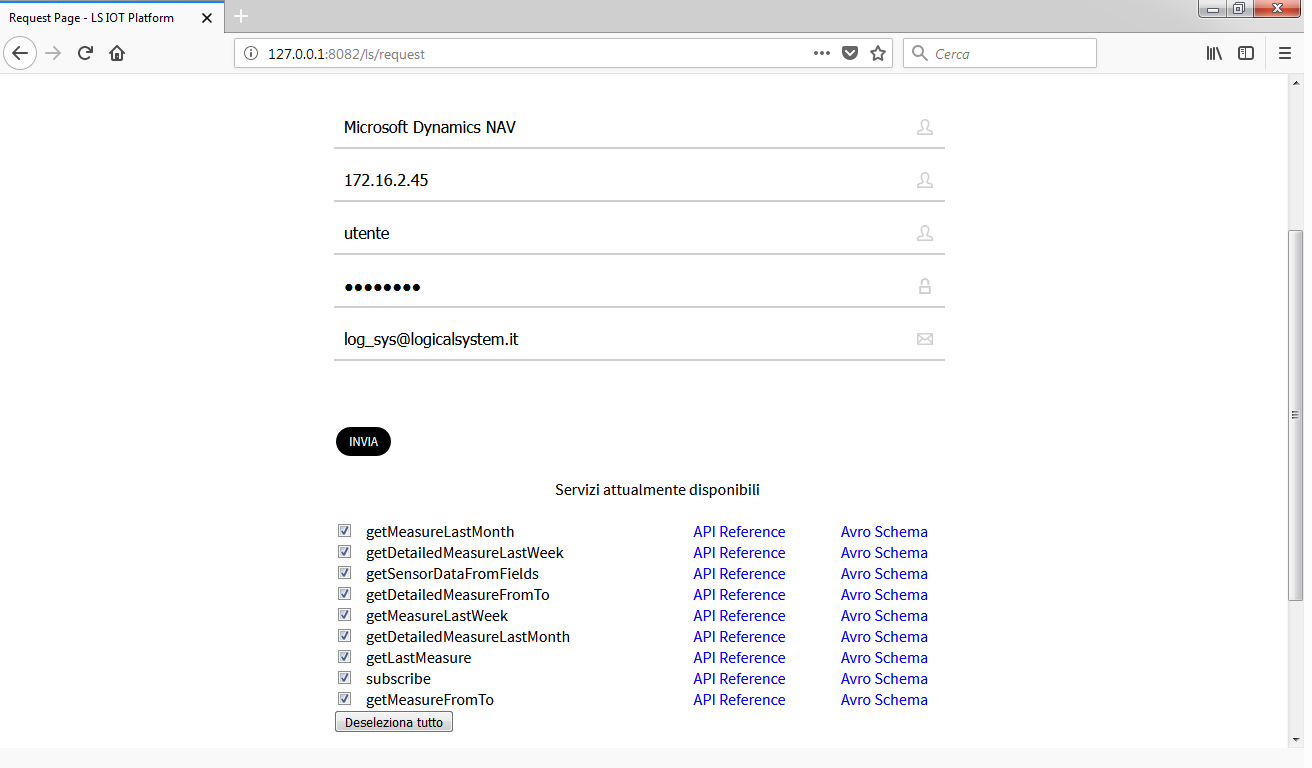
\includegraphics[width=0.9\textwidth]{images/RequestPagePlatform.png}
		\end{column}%
	\end{columns}
\end{frame}

\begin{frame}[noframenumbering]
\frametitle{LS Genio Mash-up}
\framesubtitle{Gestione (GUI)}
\begin{columns}[T] % align columns
	\begin{column}{.3\textwidth}
		
		\begin{itemize}
			{\tiny
			\item Interfaccia web richiesta abilitazione
			\item \textbf{Interfaccia web catalogo Smart Object}
			
			\begin{itemize}
				{\tiny
				\item Permette agli utenti di informarsi sulle chiamate dei servizi
				\item Descrive la misura rappresentata dai campi della tabella in Genio
				}
			\end{itemize}
			
			\item Interfaccia web gestione richieste
			\item Interfaccia web gestione servizi utenti
			%\item Interfaccia web per il real time monitoring
			%\item Interfaccia web per la gestione della soglia
			}
		\end{itemize}
	
	\end{column}%
	\hfill%
	\begin{column}{.66\textwidth}
		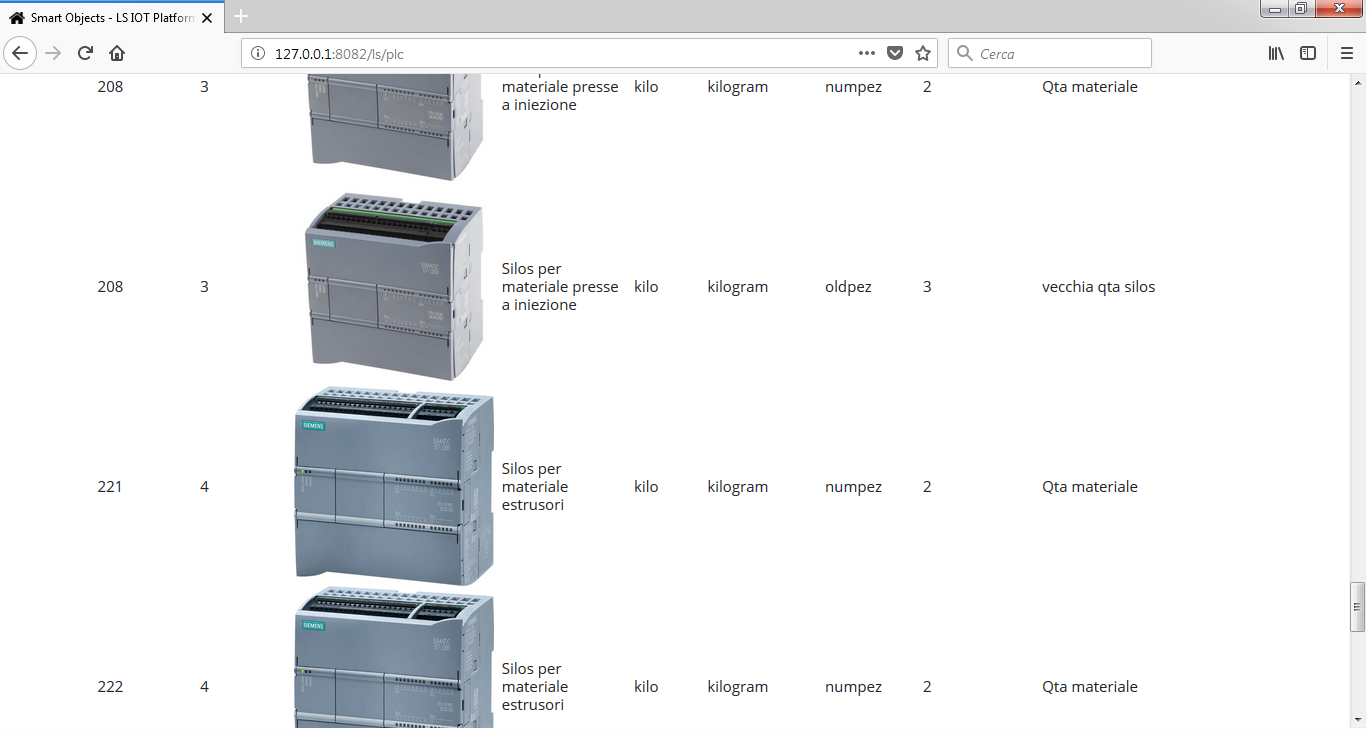
\includegraphics[width=0.9\textwidth]{images/SmartObjectsPlatform.png}
	\end{column}%
\end{columns}
\end{frame}

\begin{frame}[noframenumbering]
\frametitle{LS Genio Mash-up}
\framesubtitle{Gestione (GUI)}
\begin{columns}[T] % align columns
	\begin{column}{.3\textwidth}
		
		\begin{itemize}
			{\tiny
			\item Interfaccia web richiesta abilitazione
			\item Interfaccia web catalogo Smart Object
			\item \textbf{Interfaccia web gestione richieste}
			
			\begin{itemize}
				{\tiny
				\item Gli amministratori accettano o rifiutano richieste
				\item Viene generato il token che abilita l'uso dei servizi per quella applicazione
				}
			\end{itemize}
			
			\item Interfaccia web gestione servizi utenti
			%\item Interfaccia web per il real time monitoring
			%\item Interfaccia web per la gestione della soglia
		}
		\end{itemize}
	
	\end{column}%
	\hfill%
	\begin{column}{.66\textwidth}
		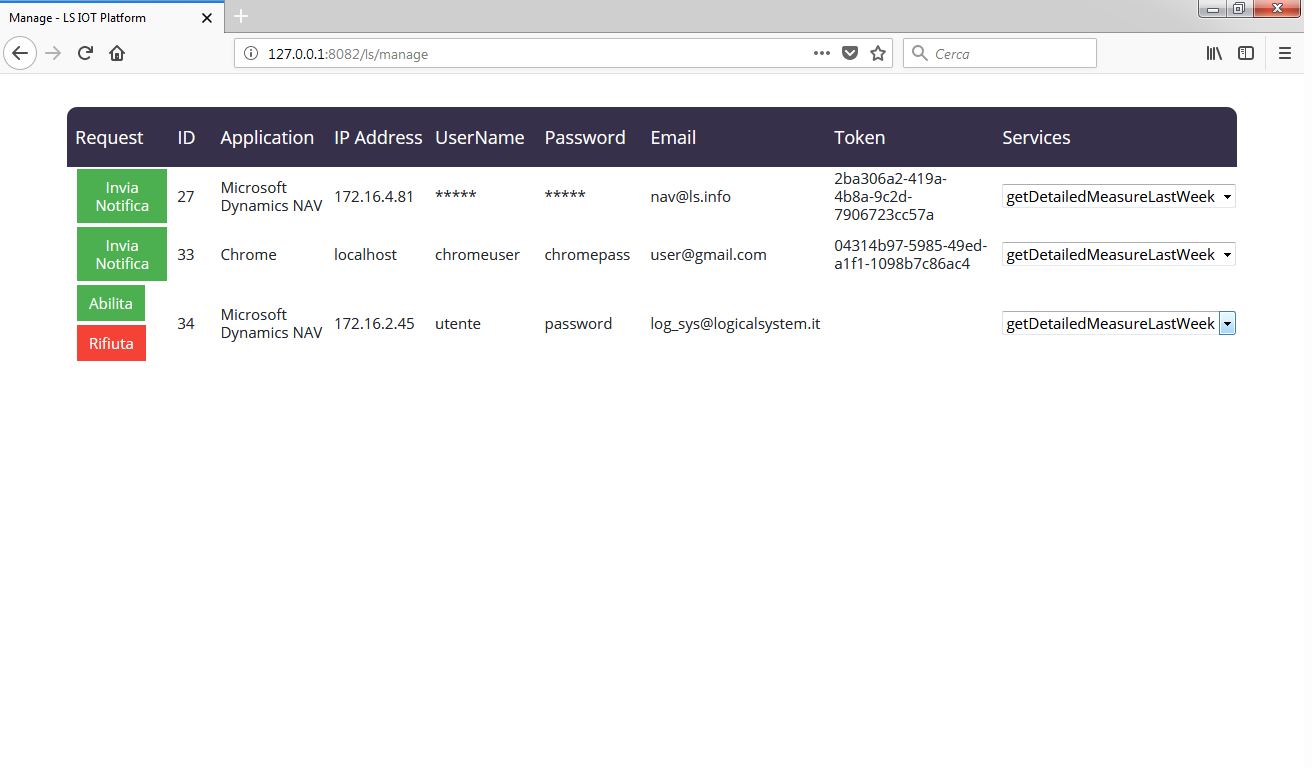
\includegraphics[width=0.9\textwidth]{images/managePagePlatform.png}
	\end{column}%
\end{columns}
\end{frame}

\begin{frame}[noframenumbering]
\frametitle{LS Genio Mash-up}
\framesubtitle{Gestione (GUI)}
\begin{columns}[T] % align columns
	\begin{column}{.3\textwidth}
		
		\begin{itemize}
			{\tiny
			\item Interfaccia web richiesta abilitazione
			\item Interfaccia web catalogo Smart Object
			\item Interfaccia web gestione richieste
			\item \textbf{Interfaccia web gestione servizi utenti}
			
			\begin{itemize}
				{\tiny
				\item Servizi attualmente attivi
				\item Attivazione di nuovi servizi
				\item Simulatore per il real time monitoring
				}
			\end{itemize}
			%\item Interfaccia web per il real time monitoring
			%\item Interfaccia web per la gestione della soglia
			}
		\end{itemize}
	
	\end{column}%
	\hfill%
	\begin{column}{.66\textwidth}
		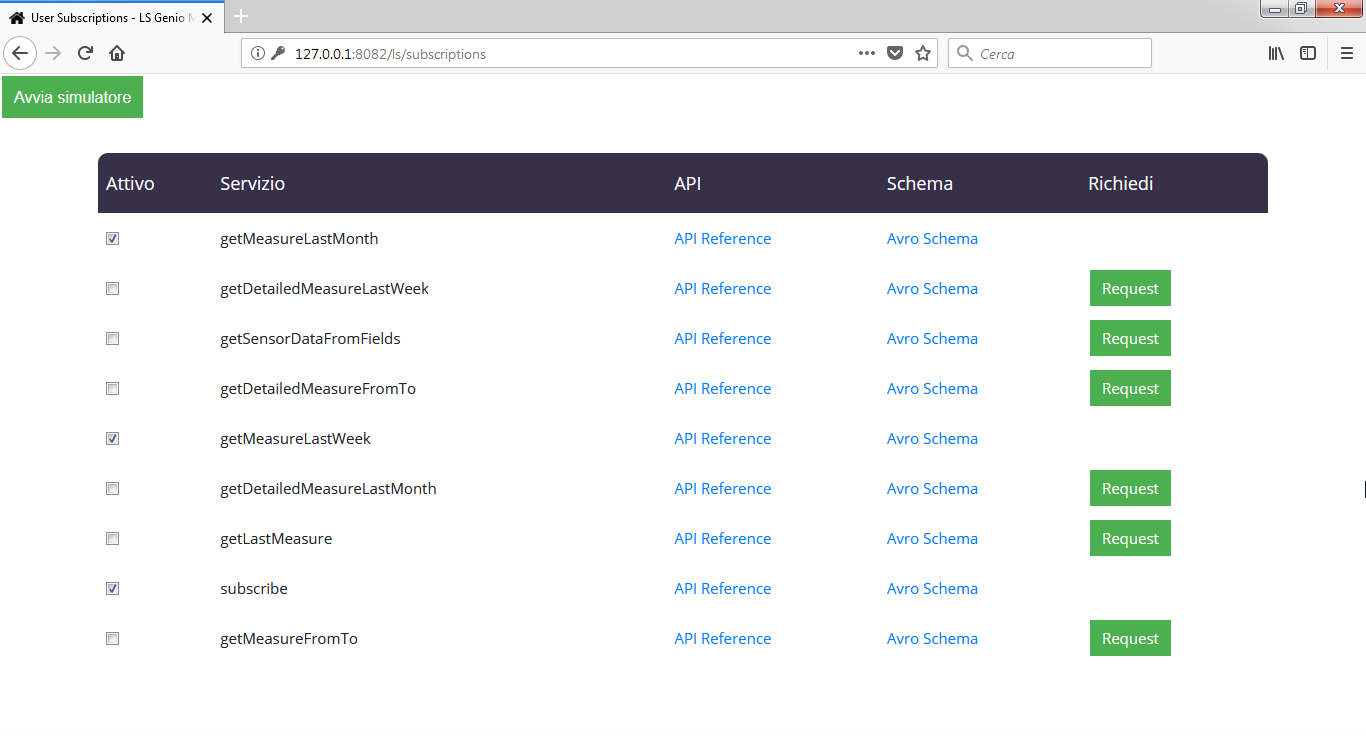
\includegraphics[width=0.9\textwidth]{images/UserSubscriptionsPlatform.png}
	\end{column}%
\end{columns}
\end{frame}



%\begin{frame}
%\frametitle{Class Diagram SubscribeRuleInterface}
%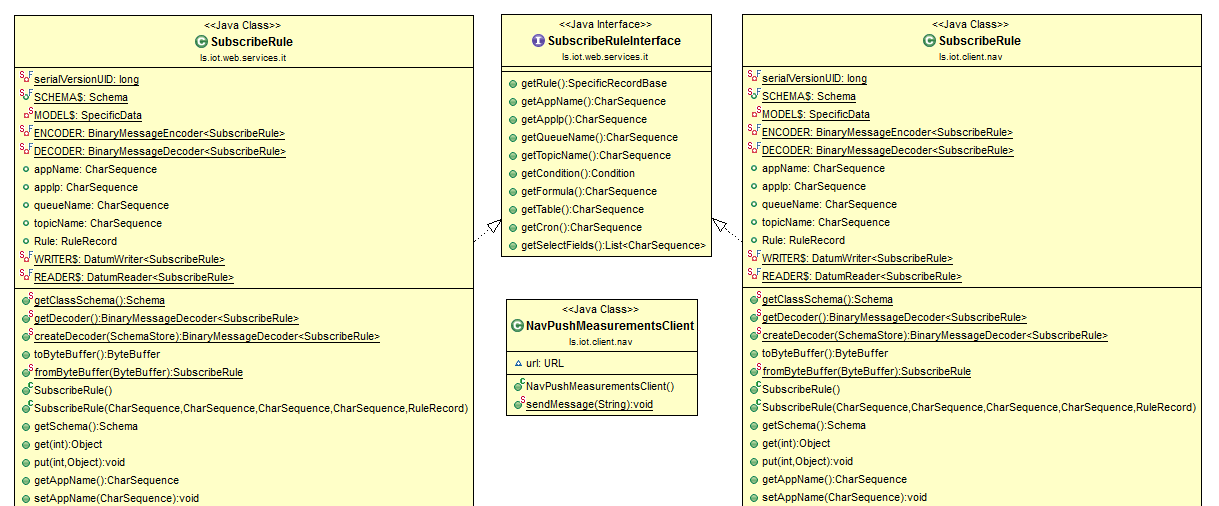
\includegraphics[width=1\textwidth]{images/figura10.png}
%\end{frame}

%\begin{frame}
%\frametitle{Class Diagram RetrievedDataInterface}
%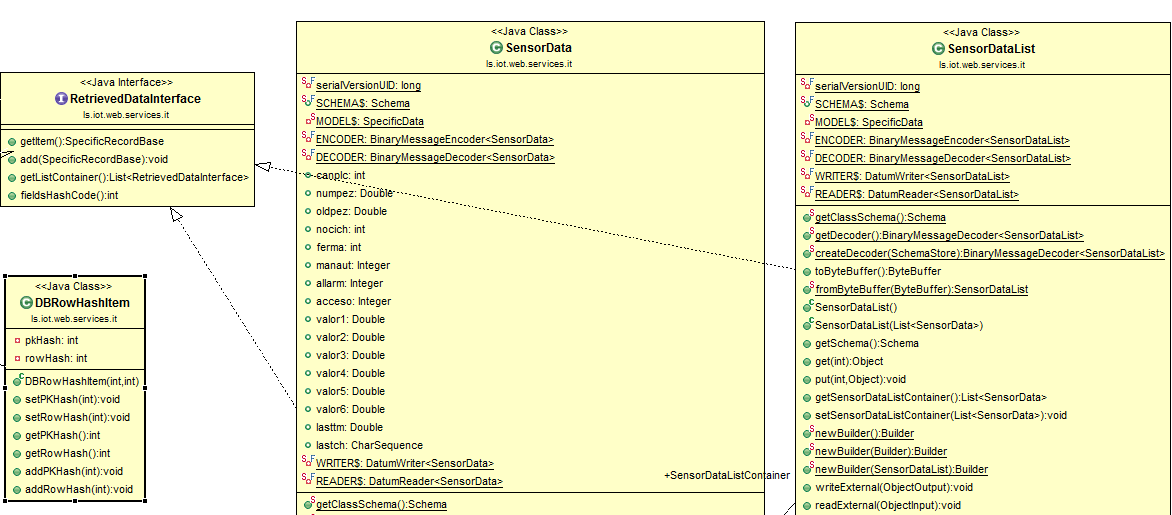
\includegraphics[width=1\textwidth]{images/ClassDiagram1.png}
%\end{frame}

%\begin{frame}
%\frametitle{Class Diagram AnnotationInterface}
%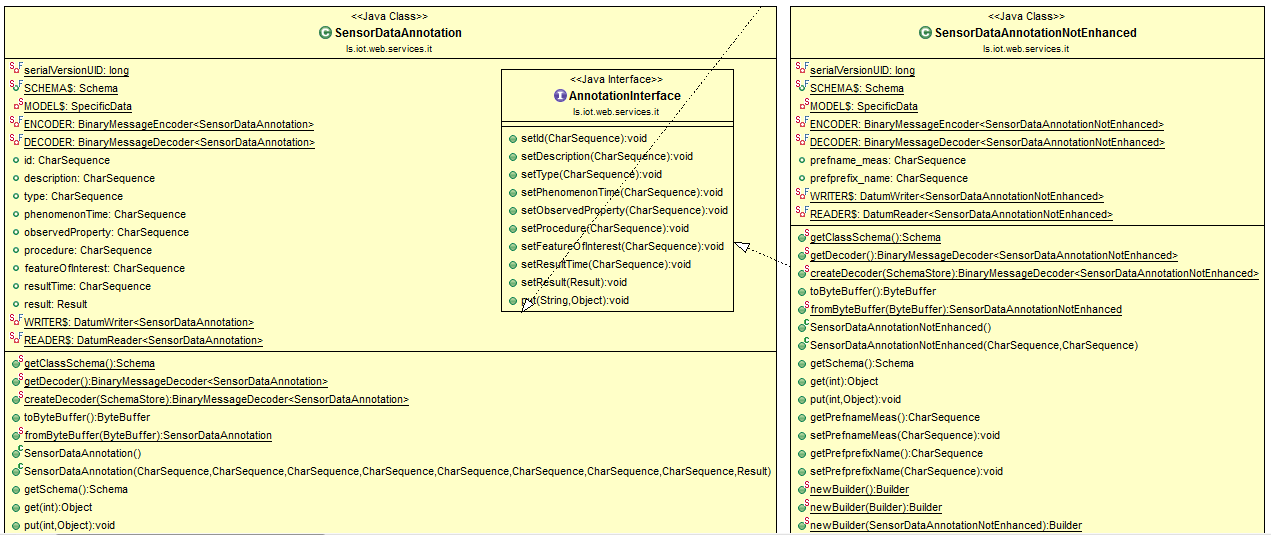
\includegraphics[width=1\textwidth]{images/annotationinterface.png}
%\end{frame}

%\begin{frame}
%\frametitle{Interfacce e classi astratte}
%\begin{columns}[T] % align columns
%	\begin{column}{.38\textwidth}
%		
%		
%	\end{column}%
%	\hfill%
%	\begin{column}{.58\textwidth}
%		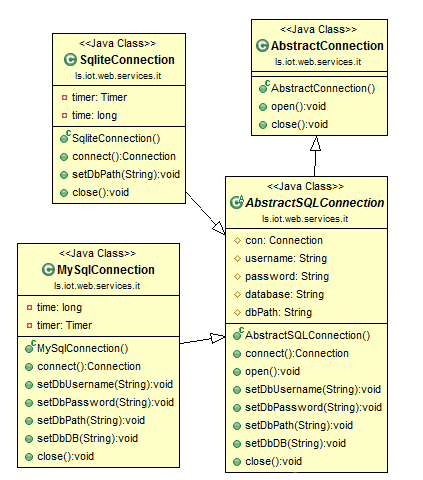
\includegraphics[width=1\textwidth]{images/classe-astratta.png}
%	\end{column}%
%\end{columns}
%
%\end{frame}

\begin{frame}
\frametitle{LS Genio Mash-up}
	\framesubtitle{Apache Avro}
	\begin{itemize}
		\item Avro: framework di serializzazione per l'interoperabilità dei dati
		\item Code generation per la gestione dei JSON
		\item Impossibilità di inviare o ricevere messaggi malformati
	\end{itemize}
\end{frame}

\begin{frame}
\frametitle{LS Genio Mash-up}
\framesubtitle{Schema Avro SensorData}
\begin{figure}%
	\centering
	\subfloat{{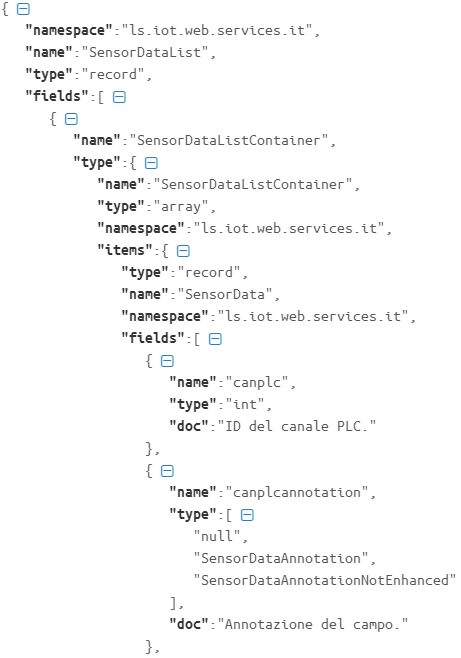
\includegraphics[width=5cm]{images/sensordata1.png} }}%
	\qquad
	\subfloat{{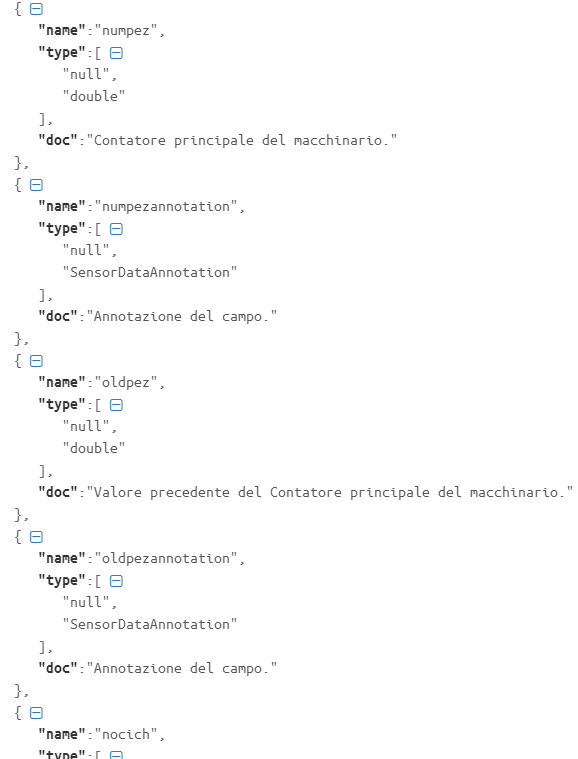
\includegraphics[width=6cm]{images/sensordata2.png} }}%
	%
	%
\end{figure}
\end{frame}

\begin{frame}
\frametitle{LS Genio Mash-up}
\framesubtitle{Schema Avro SensorDataAnnotation}
\begin{figure}%
	\centering
	\subfloat{{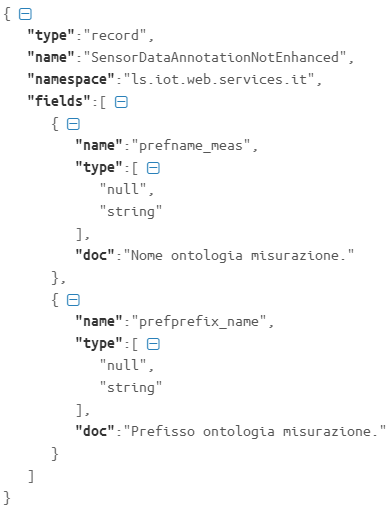
\includegraphics[width=5cm]{images/annotazione-non-avro.png} }}%
	\qquad
	\subfloat{{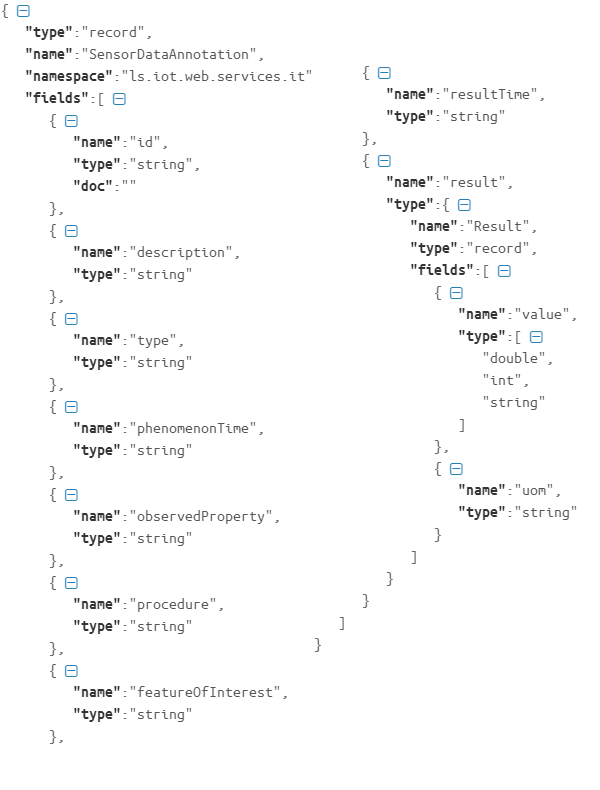
\includegraphics[width=6cm]{images/annotazione-avro.png} }}%
	%
	%
\end{figure}
\end{frame}

\begin{frame}
\frametitle{Streaming data visualization}
\framesubtitle{Interfaccia web per il real time monitoring}
\begin{columns}[T] % align columns
	\begin{column}{.3\textwidth}
		\begin{itemize}
			\small
			\item I dati che hanno una annotazione associata possono essere visualizzati
			\item PLC e campo come parametri di selezione
			\item Possibilità di avviare il controllo della soglia
		\end{itemize}
	\end{column}%
	\hfill%
	\begin{column}{.66\textwidth}
		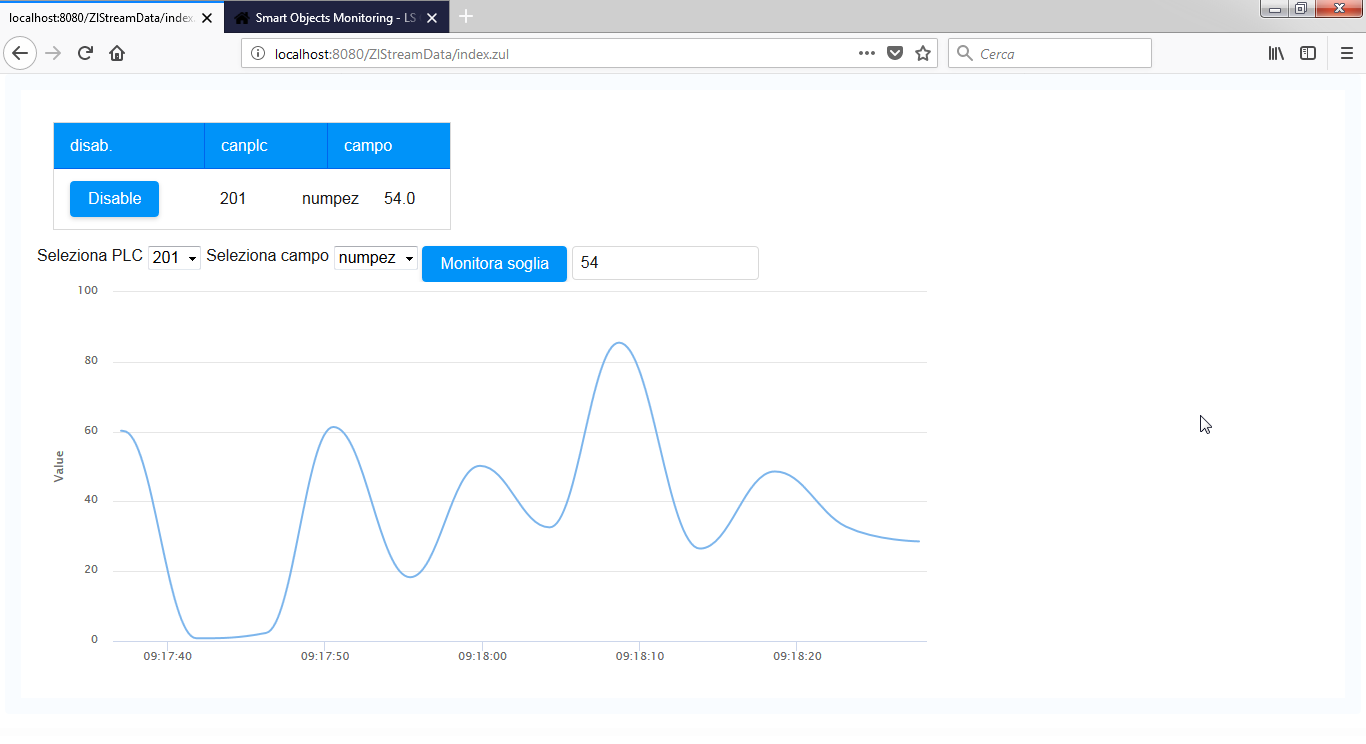
\includegraphics[width=1\textwidth]{images/grafico-zk.png}
	\end{column}%
\end{columns}

\end{frame}

\begin{frame}
\frametitle{Streaming data visualization}
\framesubtitle{Interfaccia web per il monitoring della soglia}
\begin{columns}[T] % align columns
	\begin{column}{.3\textwidth}
		\begin{itemize}
			\item Tabella con il numero di volte che la soglia è stata superata
			\item Ultima media registrata
		\end{itemize}
	\end{column}%
	\hfill%
	\begin{column}{.66\textwidth}
		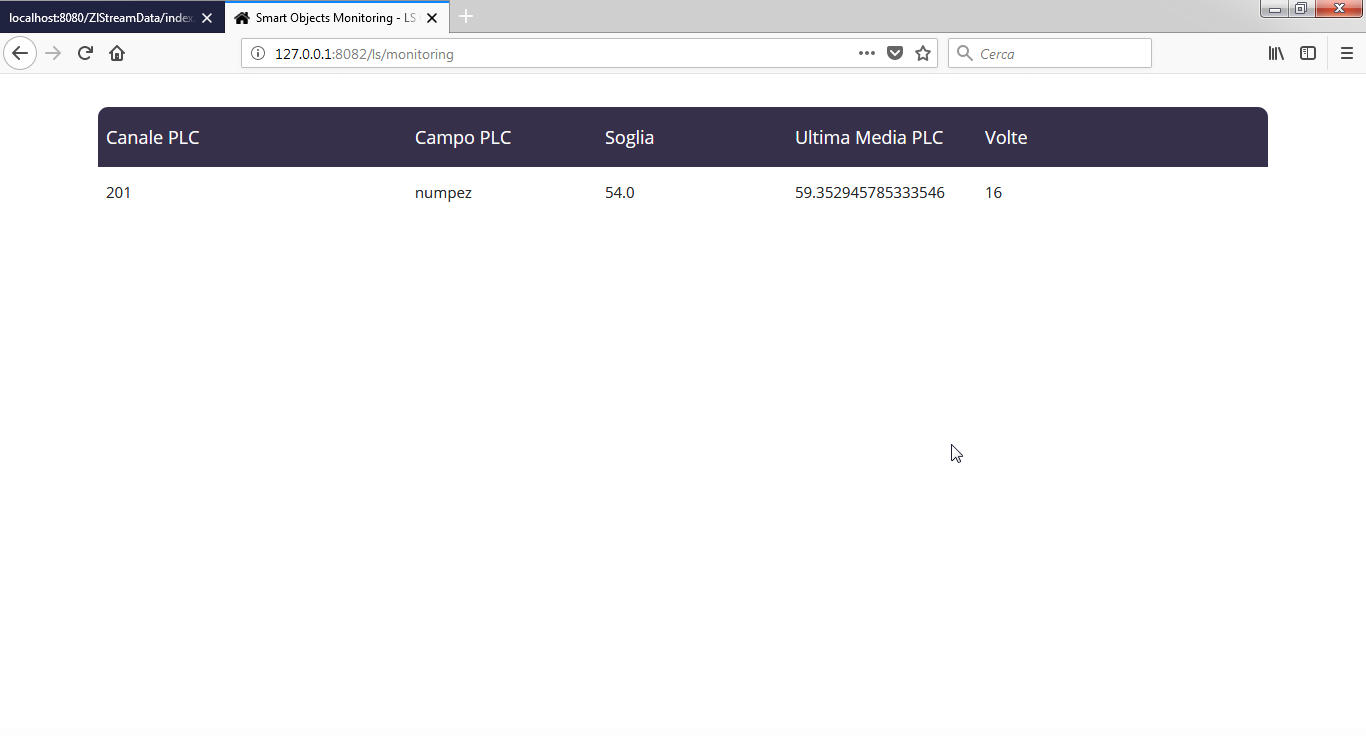
\includegraphics[width=1\textwidth]{images/pagina-monitoraggio-web.png}
	\end{column}%
\end{columns}

\end{frame}

\begin{frame}
\frametitle{Streaming data visualization}
\framesubtitle{Codice Job Flink}
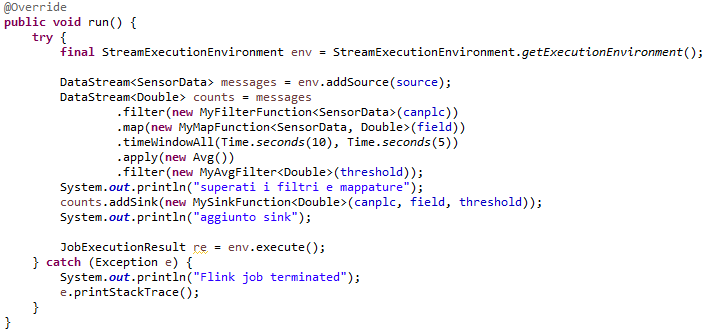
\includegraphics[width=1\textwidth]{images/flink-job.png}
\end{frame}

\begin{frame}
\frametitle{Difficoltà incontrate}
\begin{itemize}
	\item Integrazione subscribe con NAV
	\begin{itemize}
		\item Utilizzo Web Service SOAP
	\end{itemize}
\end{itemize}
\end{frame}

\begin{frame}
\frametitle{Tecnologie utilizzate}
\begin{itemize}
	\item Java
	\item Framework Jersey e Grizzly
	\item Apache Avro
	\item Apache ActiveMQ
	\item Framework ZK
	\item Apache Flink
\end{itemize}
\end{frame}

\begin{frame}
\frametitle{Risultati raggiunti}
\begin{itemize}
	\item Piattaforma indipendente
	\begin{itemize}
		\item Classi astratte e interfacce
		\item Database SQLite per autenticazione token
	\end{itemize}
	\item Servizio subscribe debolmente accoppiato
	\begin{itemize}
		\item Tramite message broker
	\end{itemize}
	\item Servizio monitoraggio dei dati
	\begin{itemize}
		\item Grafico per visualizzare andamento
		\item Apache Flink per controllo soglia
	\end{itemize}
\end{itemize}
\end{frame}

%-------------------------inizio client-----------------------------

\begin{frame}
\frametitle{Obiettivi}
\begin{itemize}
	\item Interazione di Microsoft Dynamics NAV con la piattaforma LS-Genio Mashup e definizione di un "setup" per l'utente
	%\begin{itemize}
	%	\item Mancata possibilità di consumo diretto di servizi REST
	%	\item Mancata possibilità di gestione del formato JSON
	%	\item Difficoltà nell'interazione con software esterni non Microsoft
	%\end{itemize}
	
	%\item Visualizzazione tramite NAV di un report PowerBI basato sui dati ottenuti
	
	%\item Visualizzazione da NAV di una rappresentazione grafica con PowerBI dei dati ottenuti 
	\item Realizzazione di un ontologia delle misurazioni e delle misure
\end{itemize}	
\end{frame}

\begin{frame}
\frametitle{Problematiche e risoluzioni}
\begin{itemize}
\item Software Microsoft Dynamics NAV che possiede numerose limitazioni, ostacolando l'interazione con la piattaforma
\begin{itemize}
	\item Risolto mediante implementazione di un client C\#, integrato poi su NAV
	%	\item Mancata possibilità di gestione del formato JSON
	%	\item Difficoltà nell'interazione con software esterni non Microsoft
\end{itemize}

%	\item Impossibilità di integrare un report PowerBI su NAV senza l'utilizzo di Azure
%	\begin{itemize}
%		\item Risolto mediante esportazione del report su Web
%	\end{itemize}

\item Difficoltà nel trovare un modello ontologico relativo al case study
\begin{itemize}
	\item Risolto mediante adattamento allo standard ISO 19156:2011
\end{itemize}
\end{itemize}	
\end{frame}

\begin{frame}
\frametitle{Tecnologie e software utilizzati}
\begin{itemize}
\item C\#
\item Apache Avro
\item Microsoft Dynamics NAV e C/AL code%(C/SIDE e RoleTailored Client)
\item Microsoft PowerBI
\item Protégé
\item MySQL
%\begin{itemize}
%	\item Mancata possibilità di consumo diretto di servizi REST
%	\item Mancata possibilità di gestione del formato JSON
%	\item Difficoltà nell'interazione con software esterni non Microsoft
%\end{itemize}
\end{itemize}	
\end{frame}

%\begin{frame}
%\frametitle{Client per la piattaforma}
%\begin{itemize}
%\item Sviluppato su Microsoft Dynamics NAV nonostante diverse lacune dell'ambiente
%\begin{itemize}
%\item Mancata possibilità di consumo diretto di servizi REST
%\item Mancata possibilità di gestione del formato JSON
%\item Difficoltà nell'interazione con software esterni non Microsoft
%\end{itemize}
%\item Risoluzione tramite sviluppo di un client C\#
%\begin{itemize}
%\item Con chiamata dei servizi REST, serializzazione e deserializzazione del JSON
%\item In conformità con le classi della piattaforma tramite Apache Avro
%\item Integrato poi in NAV tramite dll 
%\end{itemize}
%\item Sviluppo di un "setup" per impostare le chiamate ai servizi su NAV
%\begin{itemize}
%\item Svolto mediante 2 approcci (PLC e Machine Center)
%\item Con trattamento dei dati per l'ambiente Navision
%\item Evitando di prendere valori già inseriti o errati
%\end{itemize}
%\item Interazione con il servizio di sottoscrizione nell'ambiente NAV
%\begin{itemize}
%\item Tramite esternazione di una codeunit come web service SOAP
%\end{itemize}
%\end{itemize}
%\end{frame}

%\begin{frame}
%\frametitle{Client NAV}
%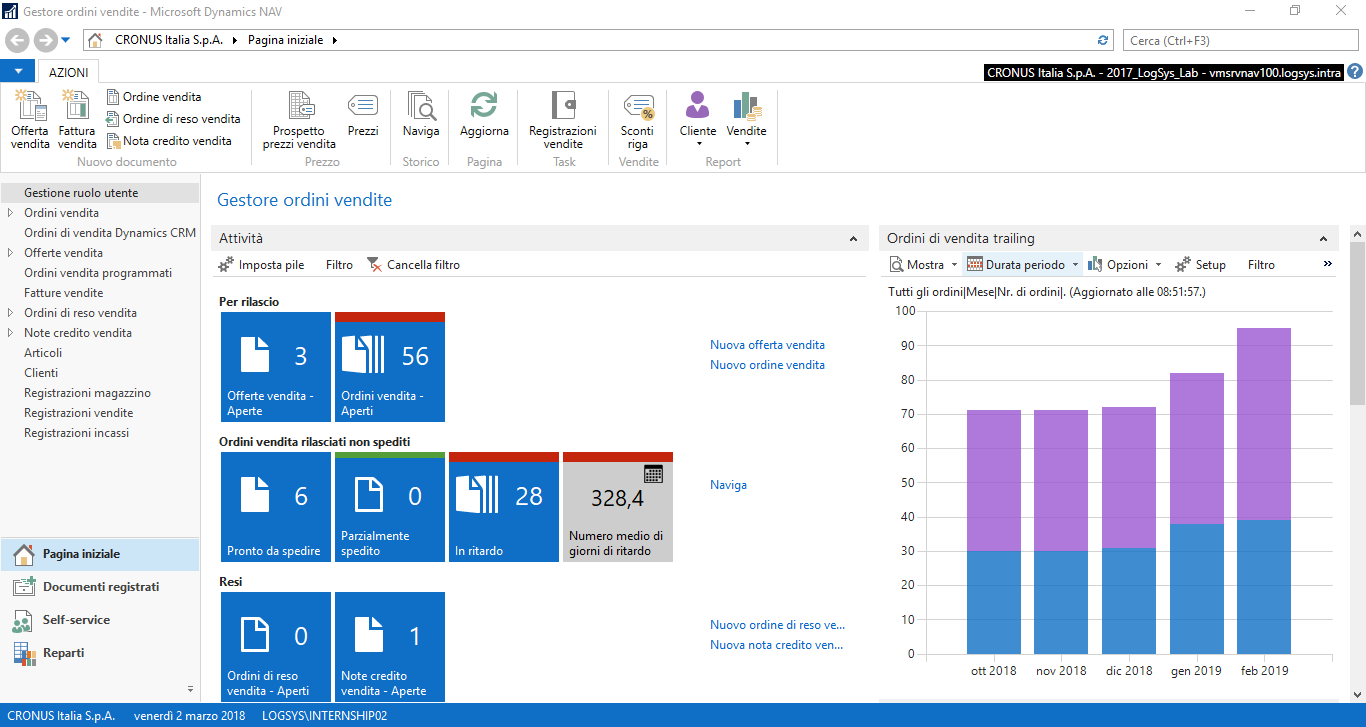
\includegraphics[width=1\textwidth]{images/NAVClient.png}
%\end{frame}

\begin{frame}
\frametitle{Class Diagram Client C\# 1}
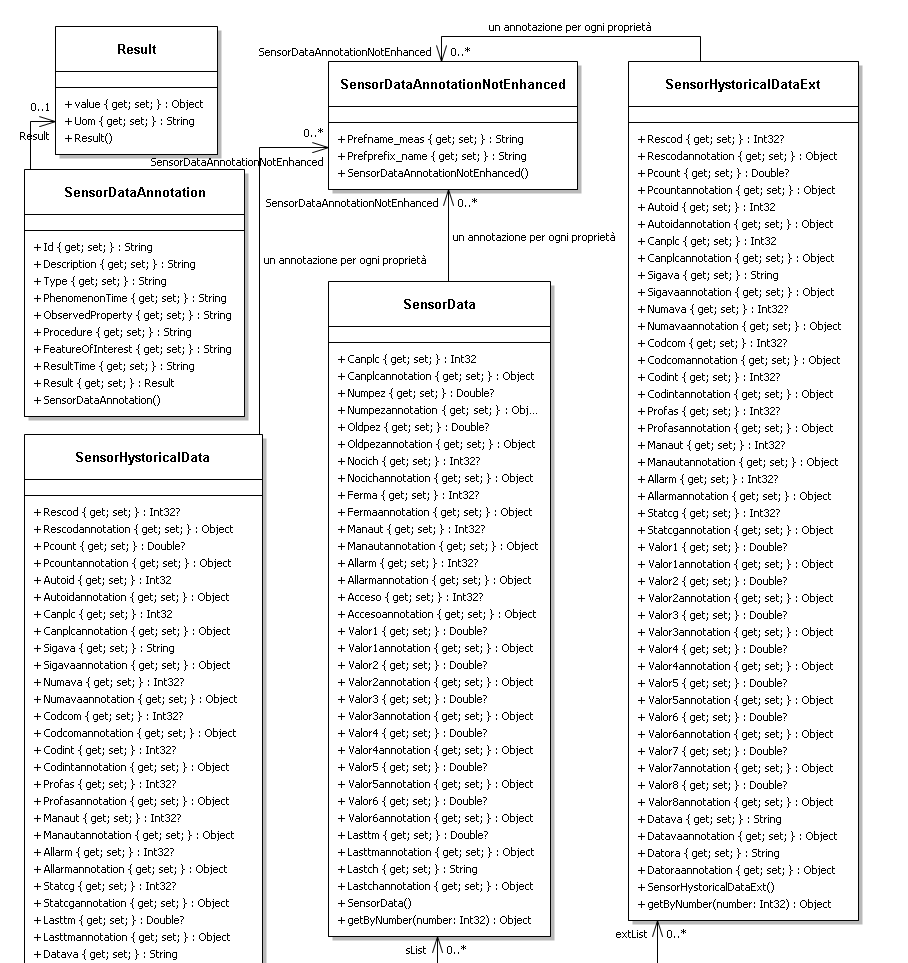
\includegraphics[width=0.65\textwidth]{images/ClassLibrary3v2part1.png}
\end{frame}

\begin{frame}
\frametitle{Class Diagram Client C\# 2}
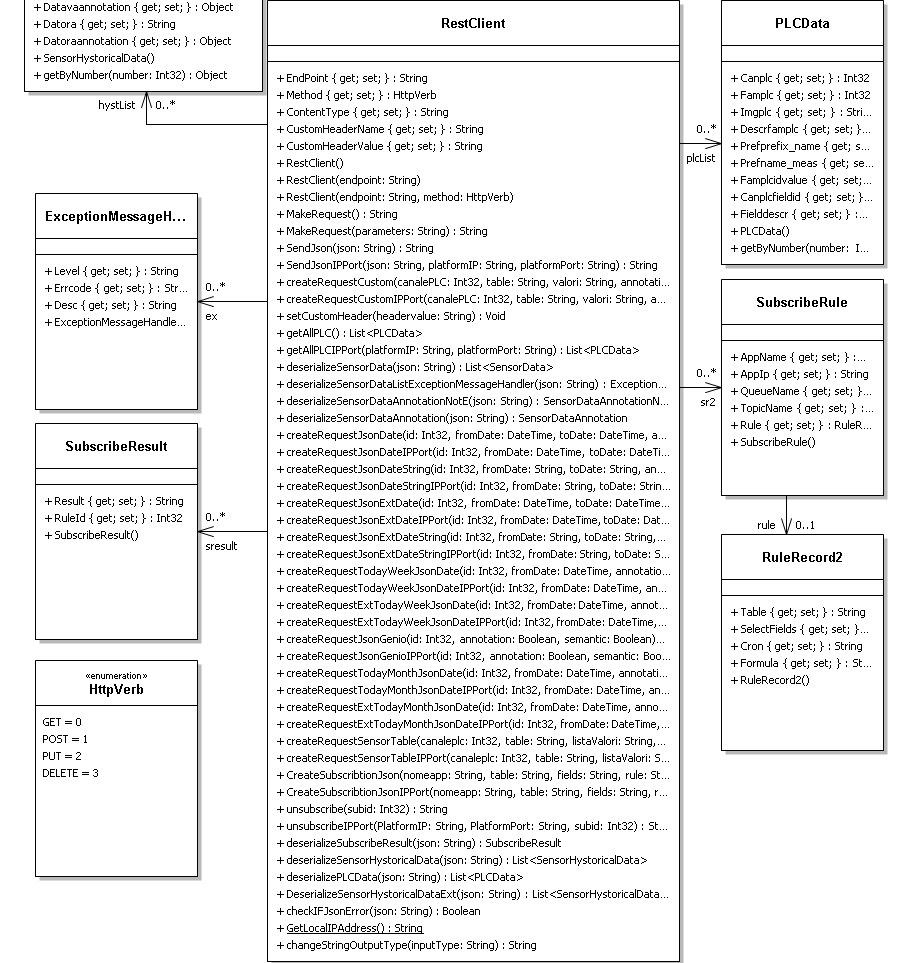
\includegraphics[width=0.65\textwidth]{images/ClassLibrary3v2part2.png}
\end{frame}

\begin{frame}
\frametitle{Ambiente di sviluppo (C/SIDE) NAV}
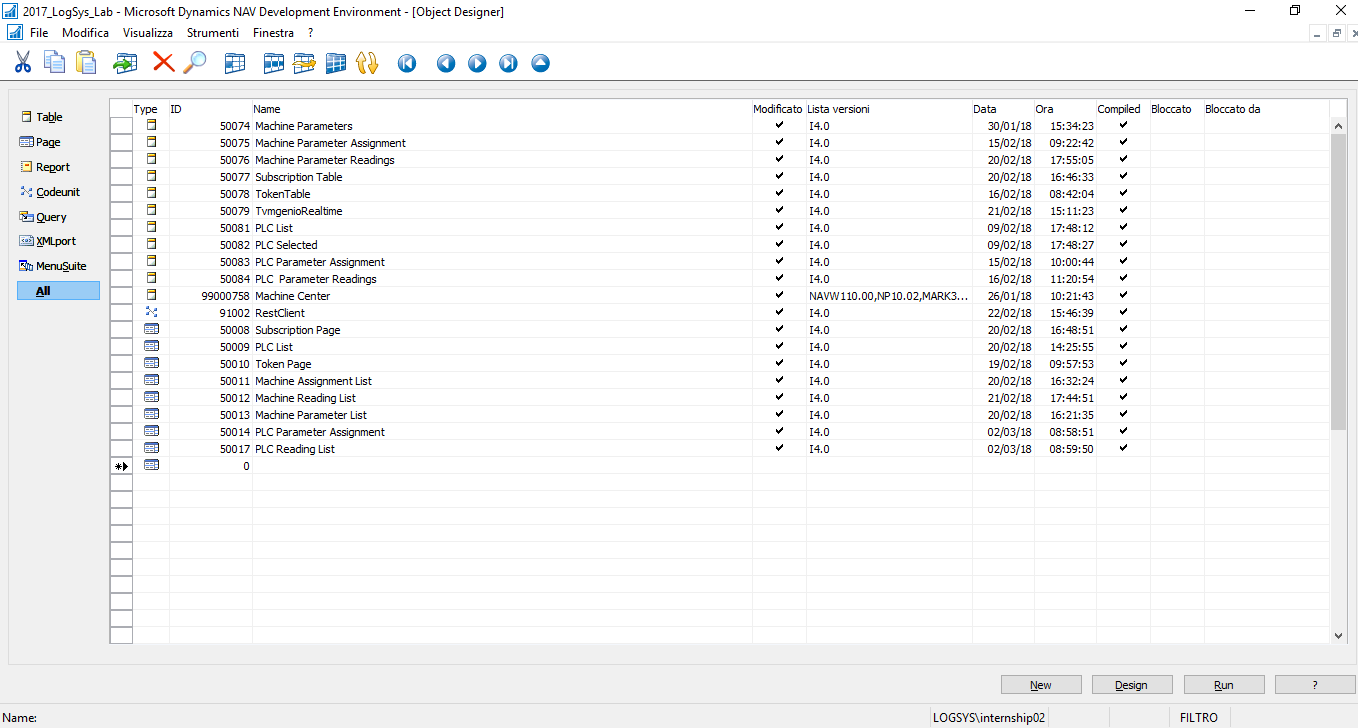
\includegraphics[width=1\textwidth]{images/NAVDevelopmentEnvironment.png}
\end{frame}


%\begin{frame}
%\frametitle{Lista delle funzioni della codeunit}
%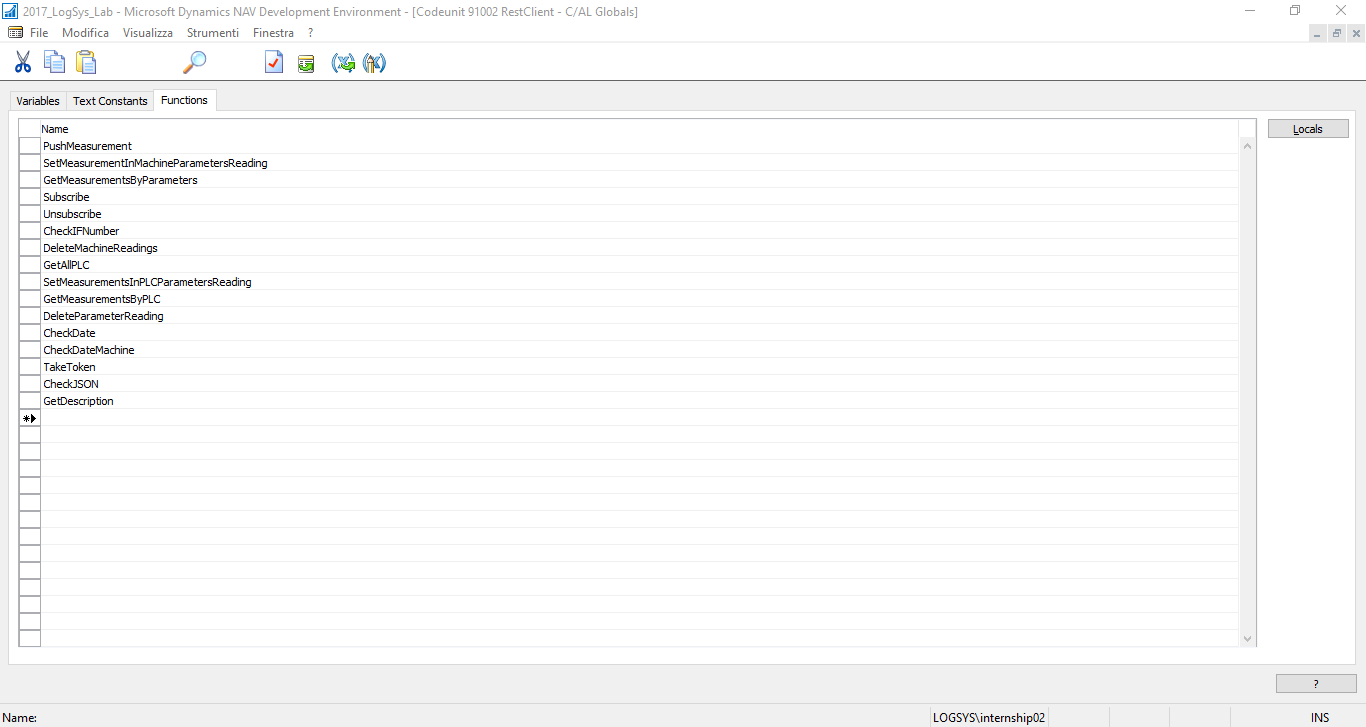
\includegraphics[width=1\textwidth]{images/NAVFunctionList.png}
%\end{frame}


%\begin{frame}
%\frametitle{La pagina Machine Center}
%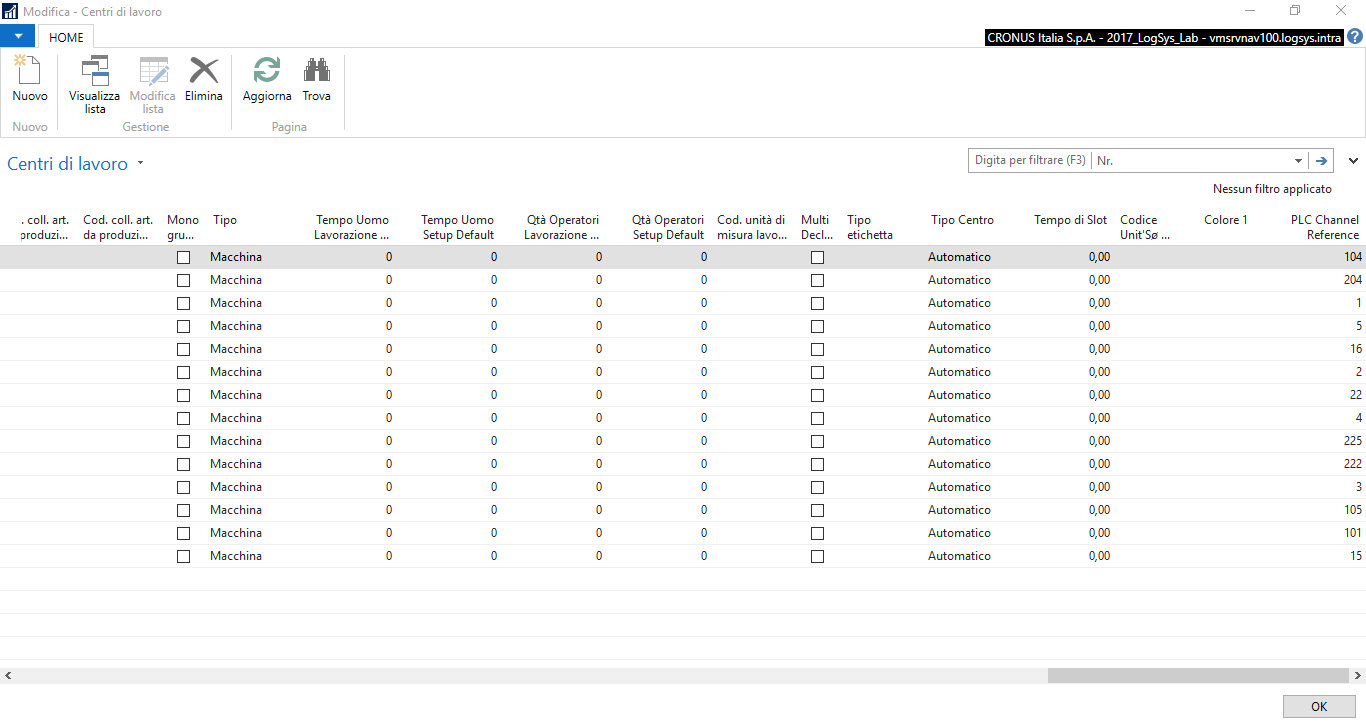
\includegraphics[width=1\textwidth]{images/MachineCenter.png}
%\end{frame}

\begin{frame}
\frametitle{La pagina Machine Assignment List}
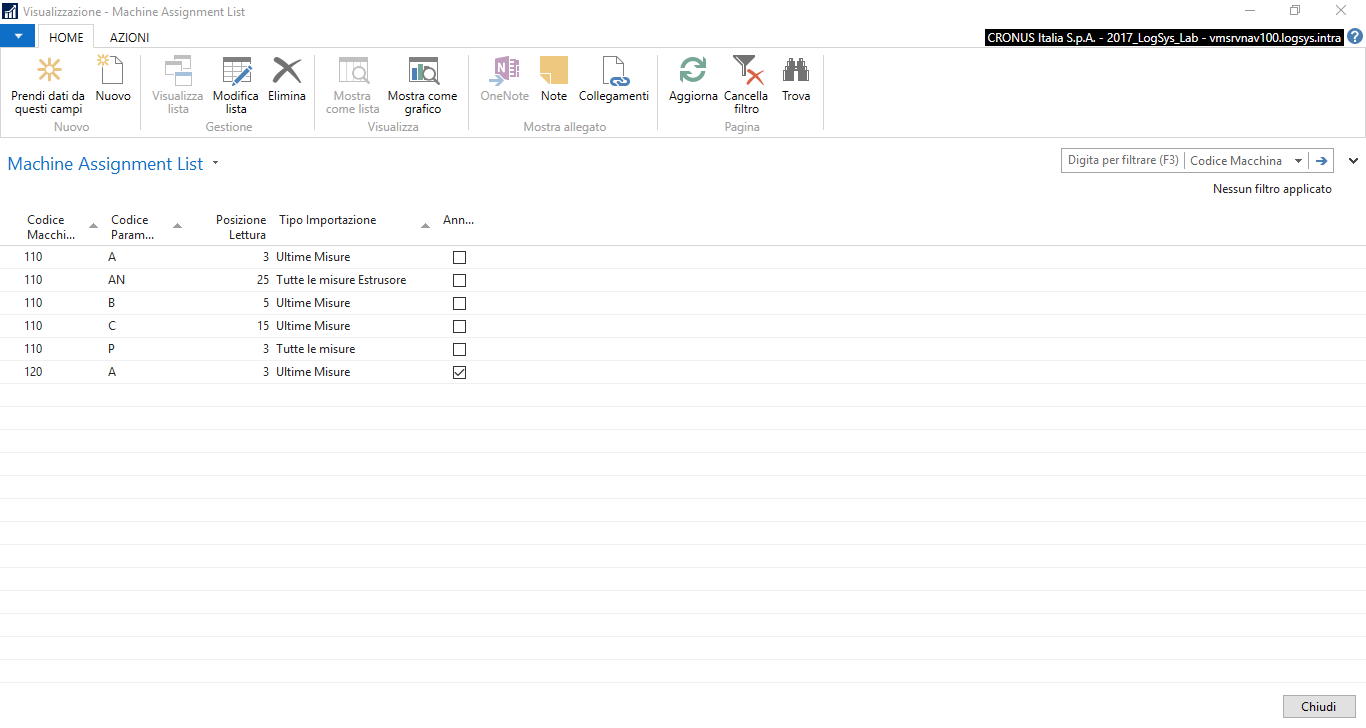
\includegraphics[width=1\textwidth]{images/MachineAssignmentList2.png}
\end{frame}


%\begin{frame}
%\frametitle{Lista con i parametri}
%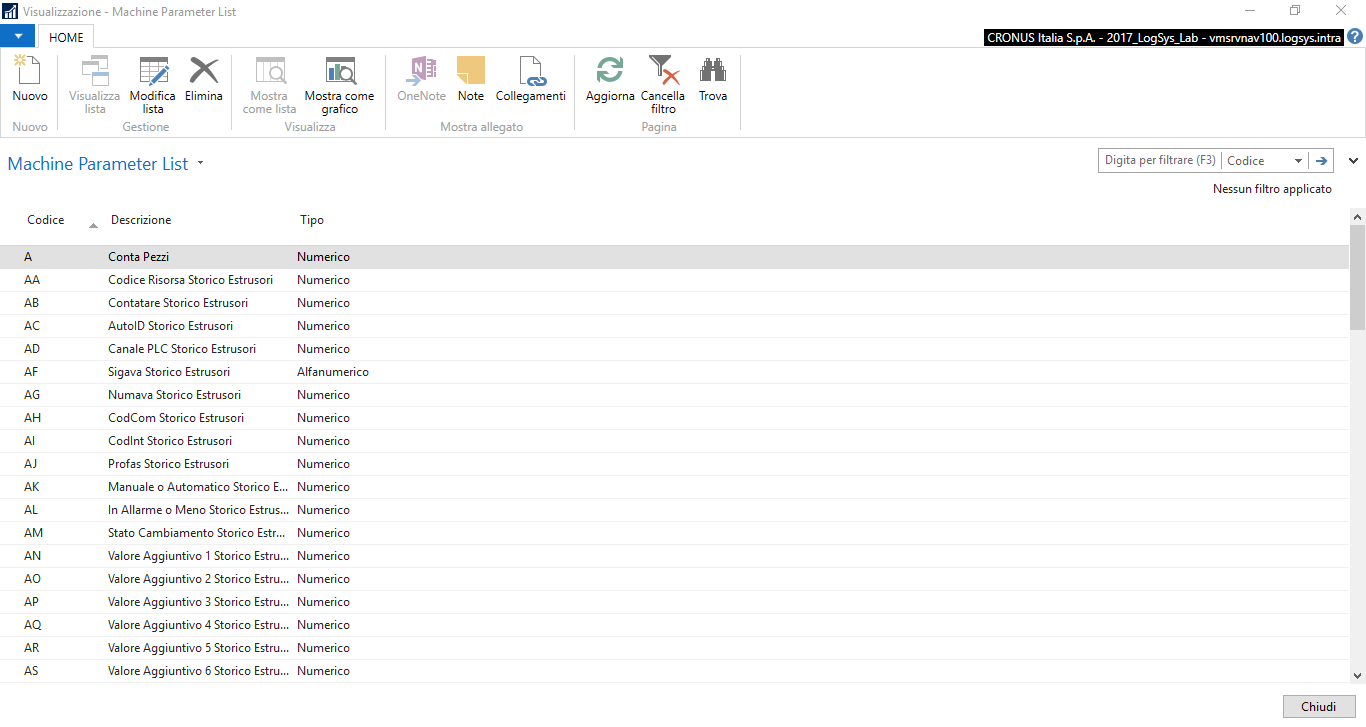
\includegraphics[width=1\textwidth]{images/MachineParameter.png}
%\end{frame}

%\begin{frame}
%\frametitle{Pagina del token}
%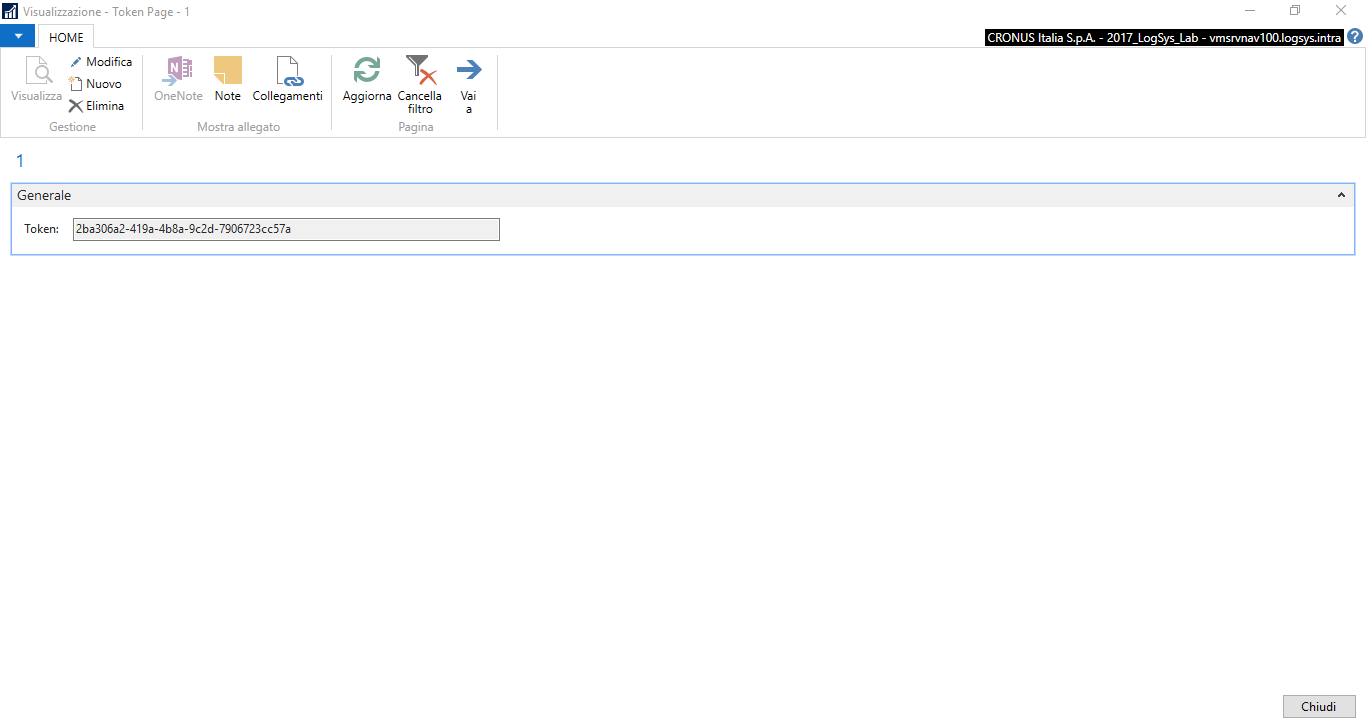
\includegraphics[width=1\textwidth]{images/tokenpage.png}
%\end{frame}



\begin{frame}
\frametitle{La pagina Machine Reading List}
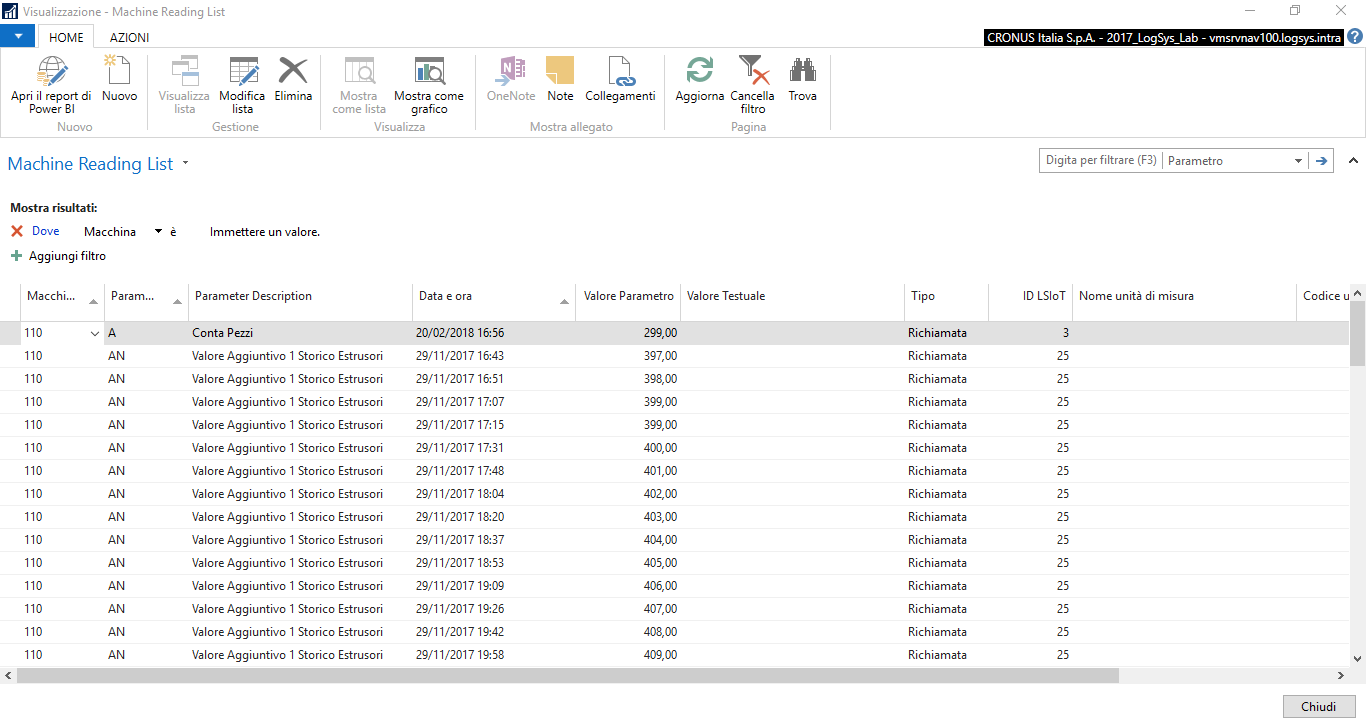
\includegraphics[width=1\textwidth]{images/MachineReadingList.png}
\end{frame}

\begin{frame}
\frametitle{Il report PowerBI nell'applicativo}
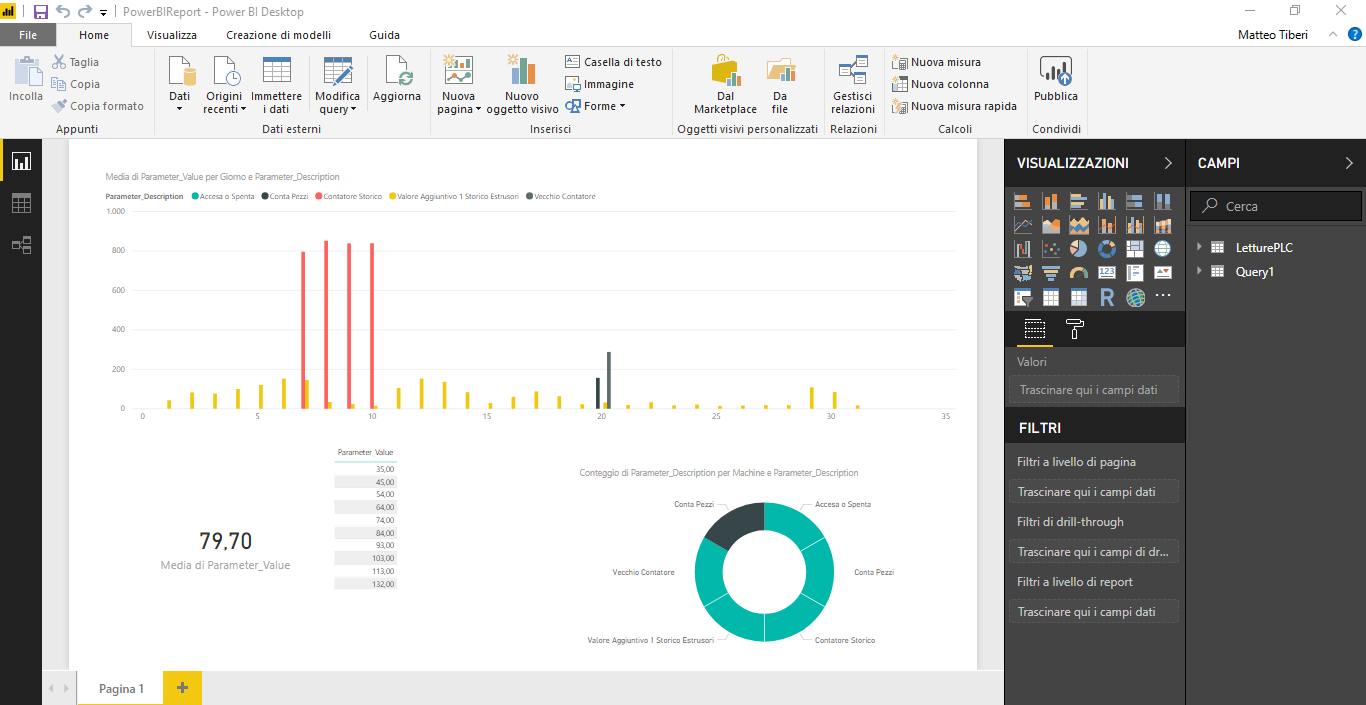
\includegraphics[width=1\textwidth]{images/PowerBI.png}
\end{frame}

\begin{frame}
\frametitle{Il report PowerBI esportato nel web}
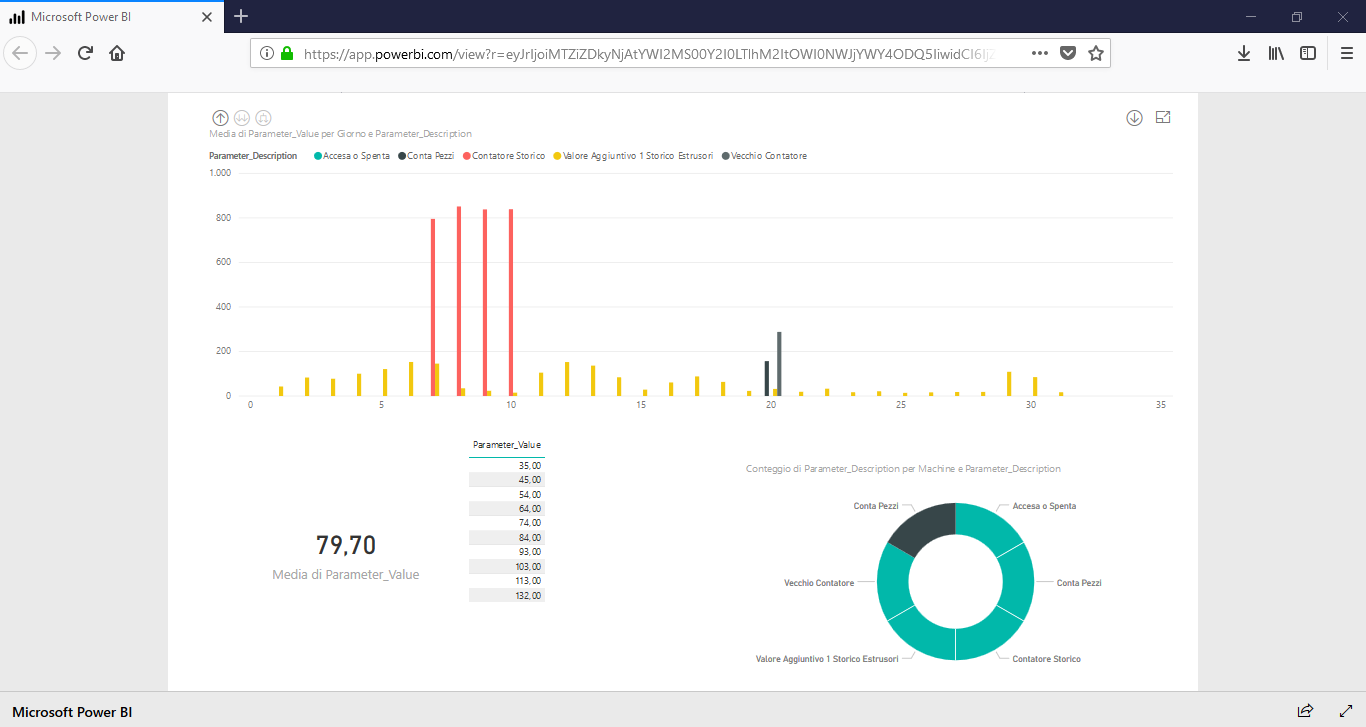
\includegraphics[width=1\textwidth]{images/ReportWEB.png}
\end{frame}

%\begin{frame}
%\frametitle{Metodo SetMeasurementPLC}
%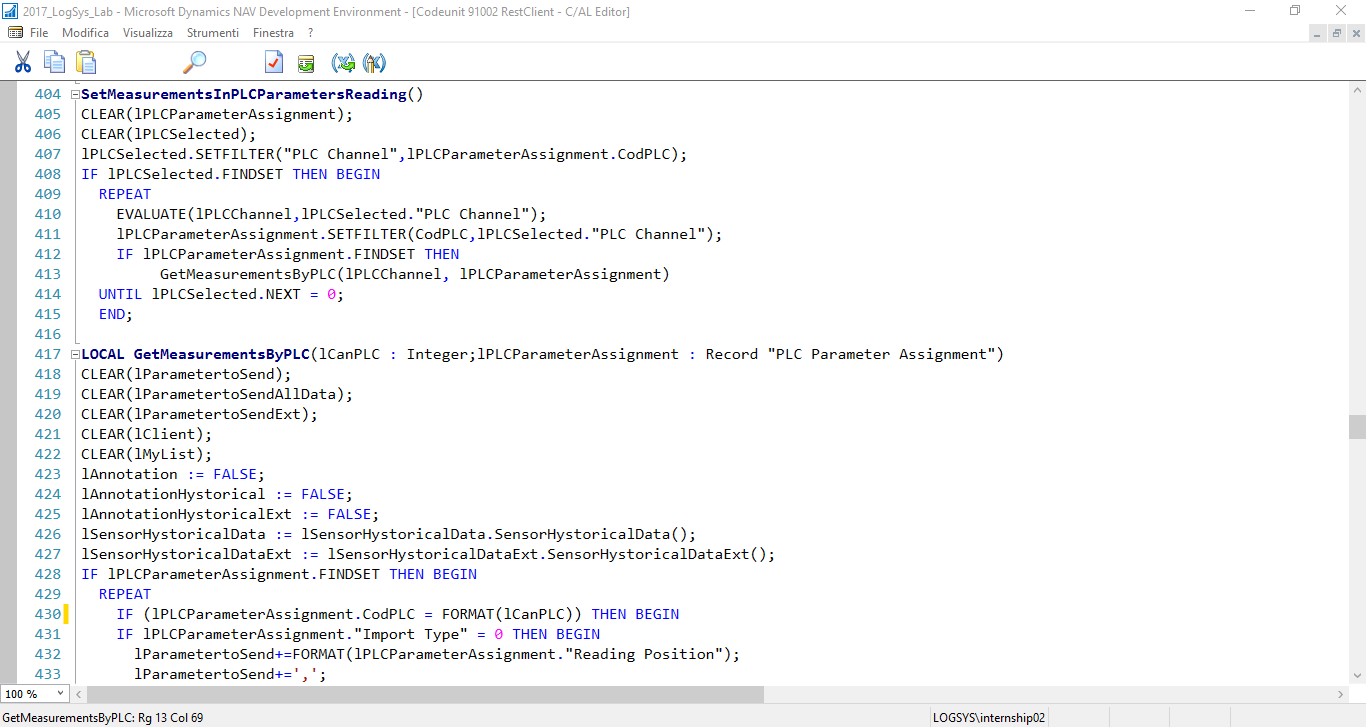
\includegraphics[width=1\textwidth]{images/NAVSetMesurament.png}
%\end{frame}

%\begin{frame}
%\frametitle{Metodo GetMeasurementPLC1}
%\includegraphics[width=1\textwidth]{images/NAVGetMesurament1.png}
%\end{frame}

%\begin{frame}
%\frametitle{Metodo GetMeasurementPLC2}
%\includegraphics[width=1\textwidth]{images/NAVGetMesurament2.png}
%\end{frame}

\begin{frame}
\frametitle{NAV servizi web}
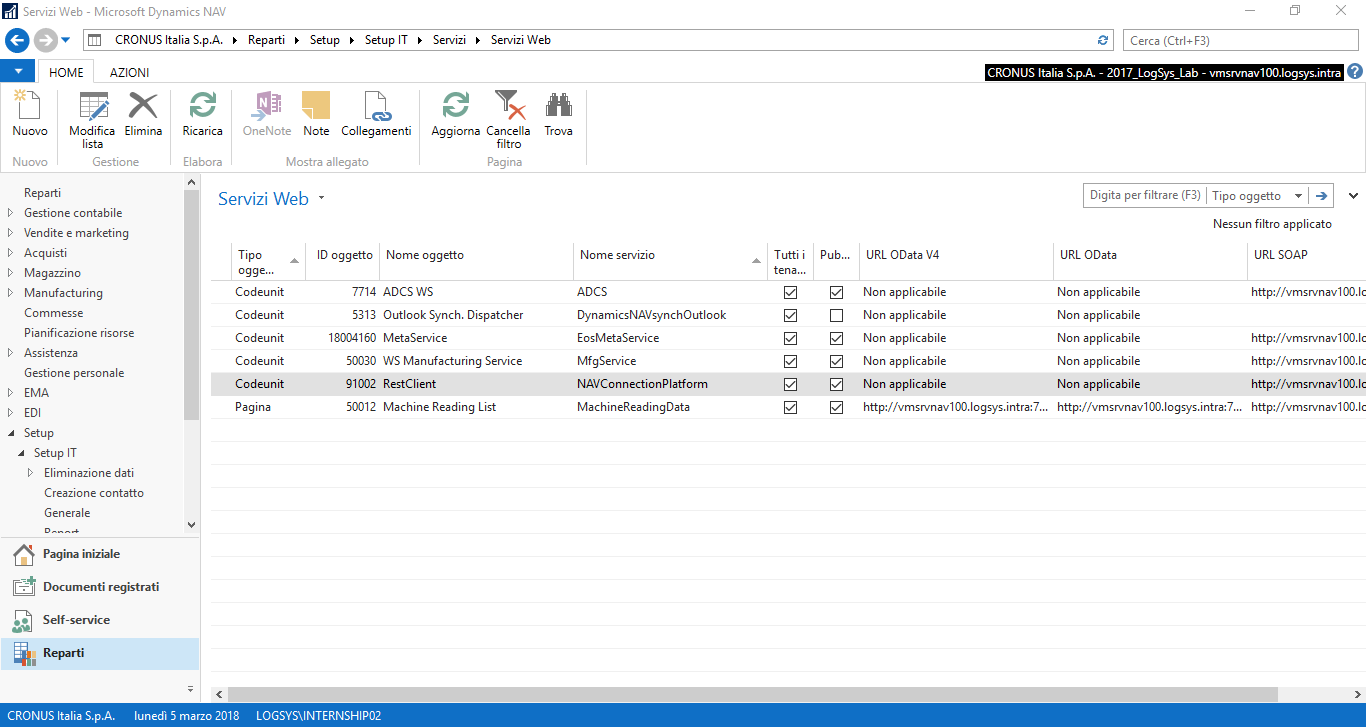
\includegraphics[width=1\textwidth]{images/NAVServiziWeb.png}
\end{frame}


\begin{frame}
\frametitle{La pagina SubscriptionPage}
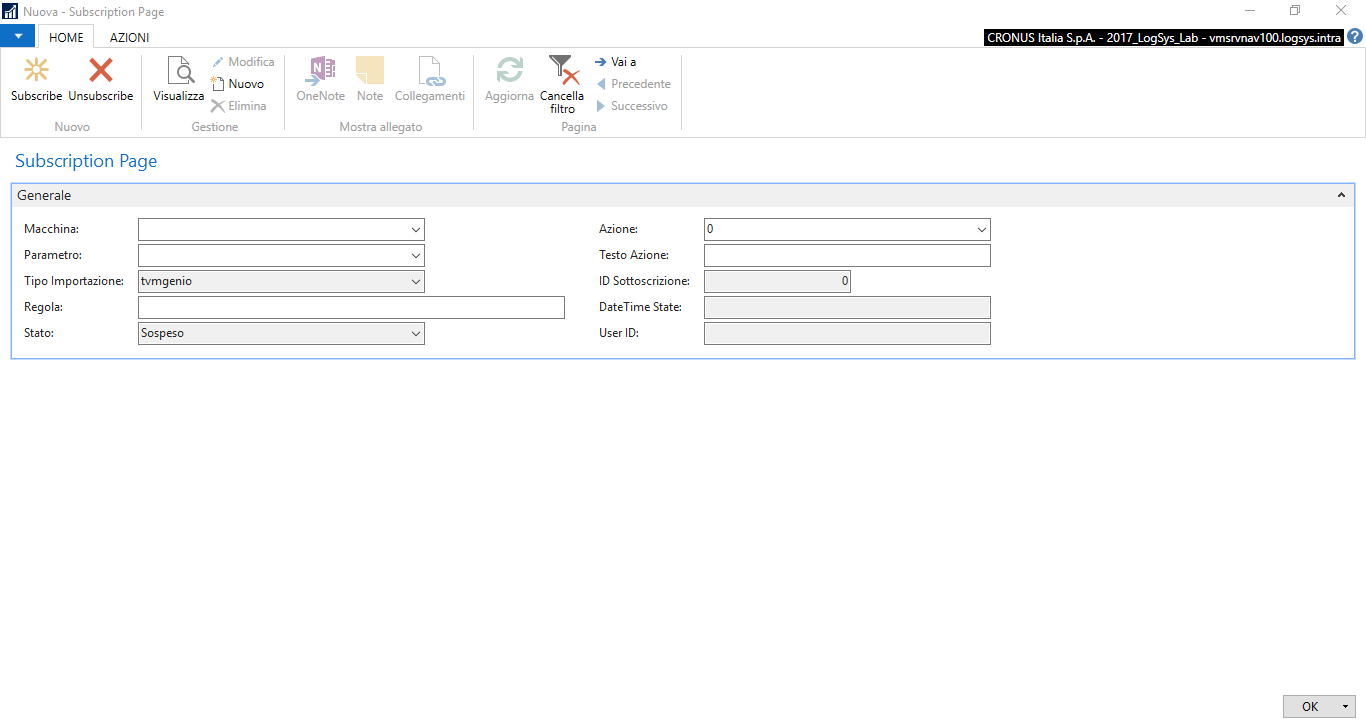
\includegraphics[width=1\textwidth]{images/NAVSubscriptionPage.png}
\end{frame}

\begin{frame}
\frametitle{Standard Observation and Measurement ISO 19156:2011}
\begin{itemize}
\item Standard basato sul concetto di osservazione, con implementazioni in formato XML e JSON
\begin{itemize}
\item Pensato per l'ambito geospaziale, il modello risulta astratto e applicabile nel case study
\end{itemize}
\item Concetto di osservazione generico specializzato in base al risultato (es. Measurement)
\begin{itemize}
%\item All'interno del case study non tutte le specializzazioni proposte vengono utilizzate
\item Solo alcune specializzazioni sono utilizzate nel case study
\end{itemize}
\item Al risultato di una osservazione specializzata viene poi associata un ontologia delle misure
\end{itemize}	
\end{frame}

\begin{frame}
\frametitle{Tabelle backend annotazioni}
\includegraphics[width=1\textwidth]{images/AltreTabelleAnnotazioniMOD4.png}
\end{frame}

%\begin{frame}
%\frametitle{Metodo PushMeasurement 1}
%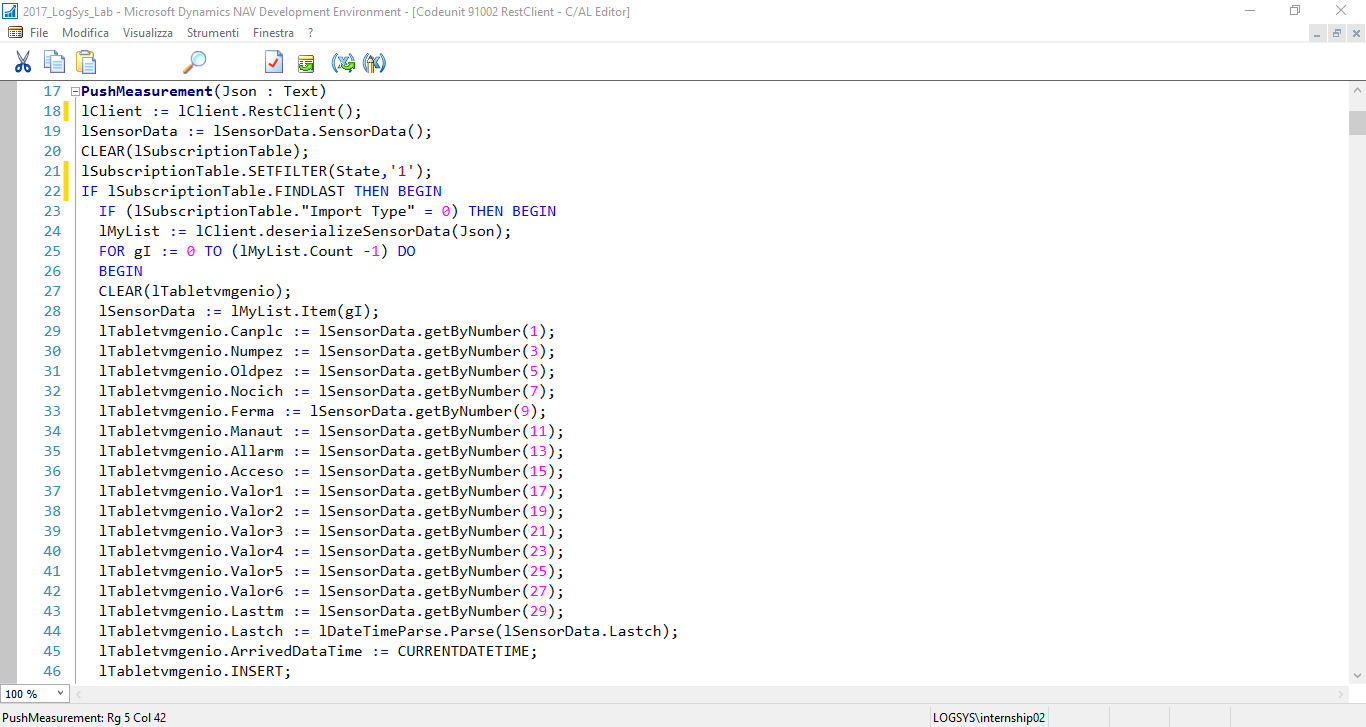
\includegraphics[width=1\textwidth]{images/NAVPushMeasuraments1.png}
%\end{frame}

%\begin{frame}
%\frametitle{Metodo PushMeasurement 2}
%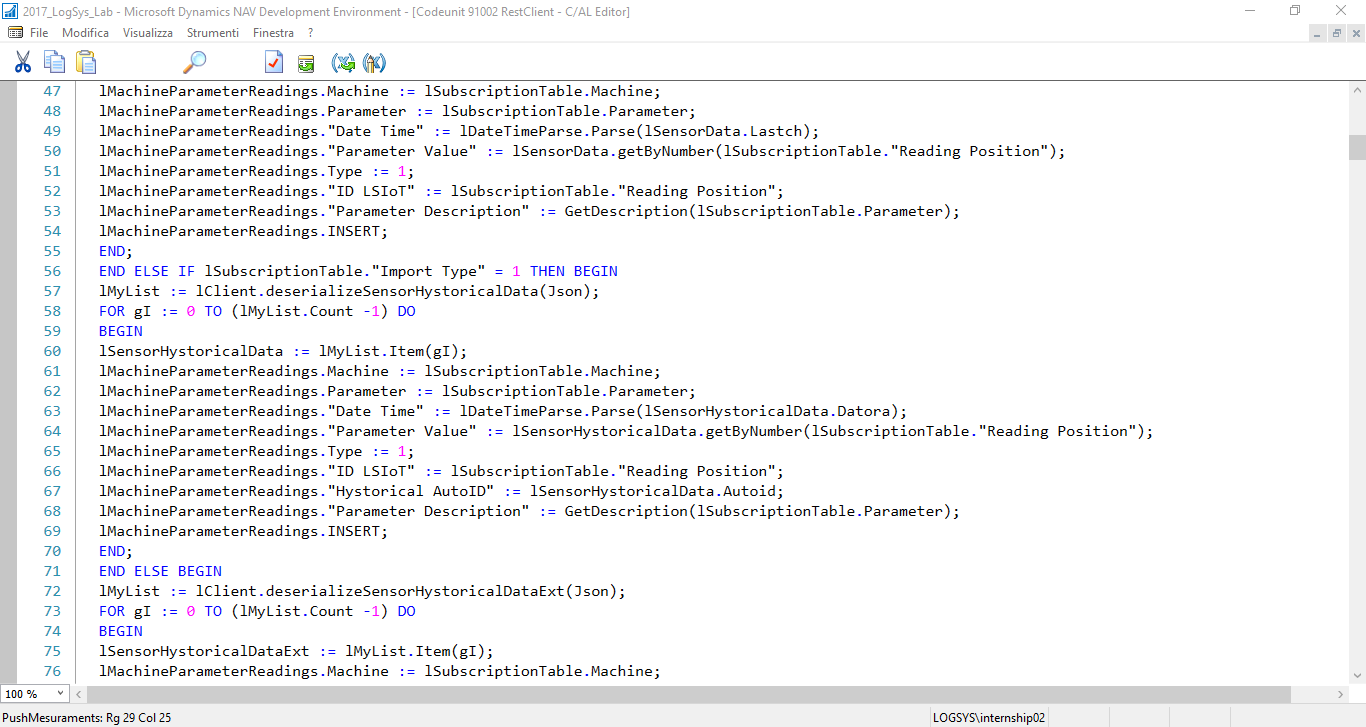
\includegraphics[width=1\textwidth]{images/NAVPushMeasuraments2.png}
%\end{frame}

%\begin{frame}
%\frametitle{Metodo PushMeasurement 3}
%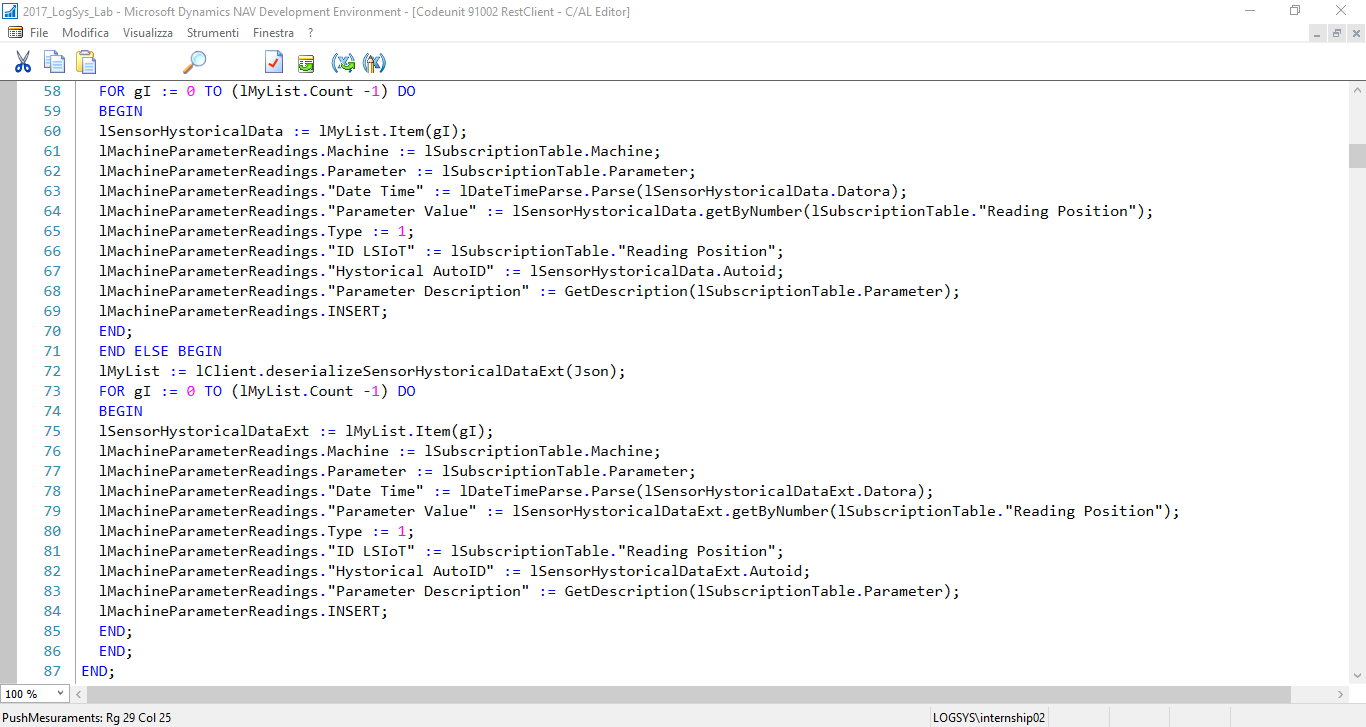
\includegraphics[width=1\textwidth]{images/NAVPushMeasuraments3.png}
%\end{frame}

\begin{frame}
\frametitle{Esempio XML}
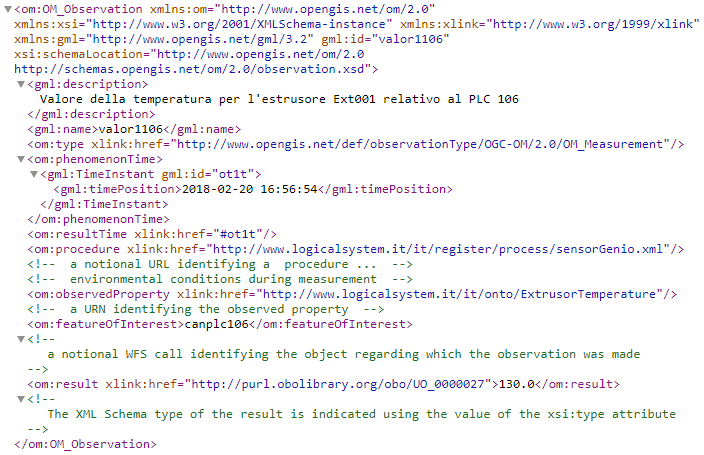
\includegraphics[width=1\textwidth]{images/TemperatureXML2.png}
\end{frame}

\begin{frame}
\frametitle{Esempio JSON}
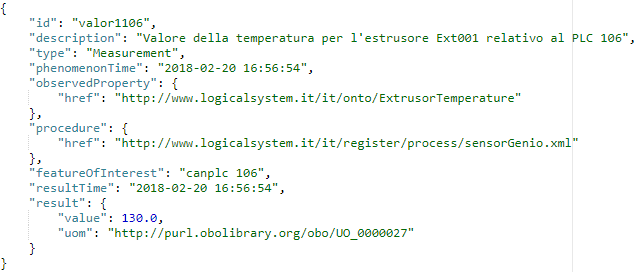
\includegraphics[width=1\textwidth]{images/TemperatureJSON.png}
\end{frame}

\begin{frame}
\frametitle{Grafico misurazioni e misure}
\begin{figure}%
%\centering
\subfloat{{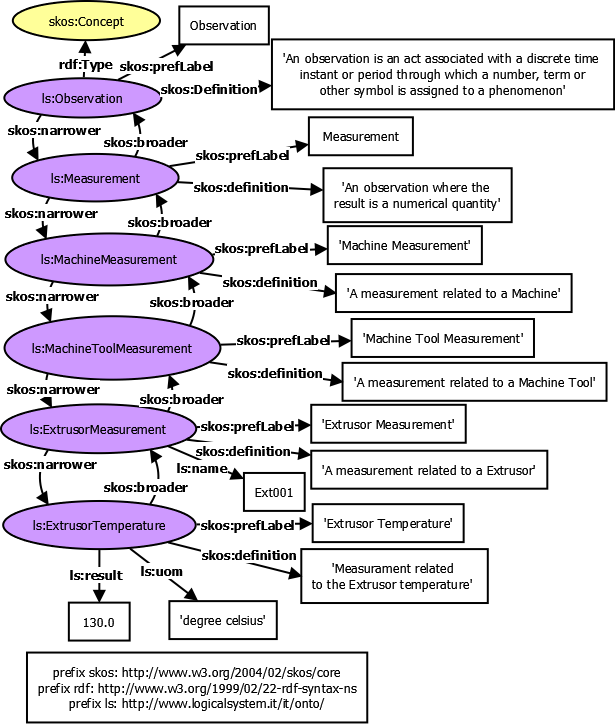
\includegraphics[width=0.565\columnwidth]{images/TempExample2.png} }}%
%\qquad
\hfill
\subfloat{{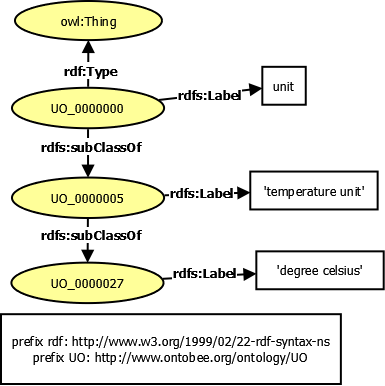
\includegraphics[width=5cm]{images/celsius.png} }}%
%
%
\end{figure}
\end{frame}

%\begin{frame}
%\frametitle{Grafico Misurazioni}
%\begin{center}
%	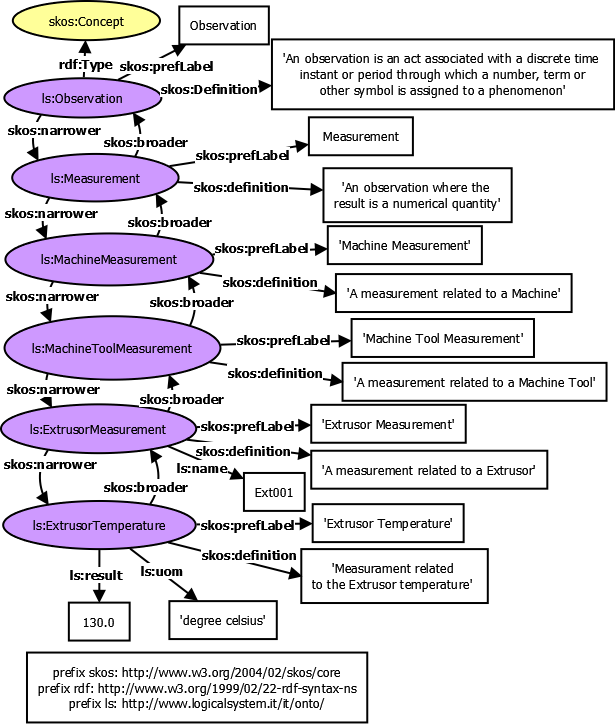
\includegraphics[width=0.6\textwidth]{images/TempExample2.png}
%\end{center}
%\end{frame}

%\begin{frame}
%\frametitle{Grafico Misure}
%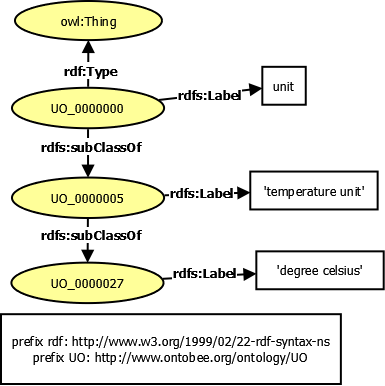
\includegraphics[width=0.6\textwidth]{images/celsius.png}
%\end{frame}

\begin{frame}
\frametitle{Pagina web ExtrusorTemperature}
\includegraphics[width=1\textwidth]{images/ExtrusorTemperature2.png}
\end{frame}

%\begin{frame}
%\frametitle{JSON con annotazione semantica}
%\includegraphics[width=1\textwidth]{images/JSONRestituito.png}
%\end{frame}


\begin{frame}
\frametitle{Conclusioni}
\begin{itemize}
\item L'integrazione tra NAV e la piattaforma ha avuto esito positivo tramite uso del client C\# 
\begin{itemize}
\item Permettendo agli utenti un semplice utilizzo dei servizi
\end{itemize}
%\item Il report PowerBI è disponibile tramite NAV
%\begin{itemize}
%	\item Permettendo agli utenti una visualizzazione grafica dinamica dei dati ricevuti
%\end{itemize}
\item L'ontologia delle misurazioni e delle misure è stata implementata
\begin{itemize}
\item In modo da avere una descrizione dei dati ottenuti dai servizi
\end{itemize}

\end{itemize}	
\end{frame}


\end{document}